%% The openany option is here just to remove the blank pages before a new chapter
\documentclass[11pt,openany]{book}
\usepackage[utf8]{inputenc}
\usepackage{subcaption}
\usepackage{graphicx}
\usepackage{kantlipsum}
\usepackage{amsfonts}
\usepackage{amsmath}
\usepackage{float}
\usepackage{algorithm}
\usepackage{algorithmic}
\usepackage{hyperref}
\usepackage{tabularx}
\usepackage{diagbox}
\usepackage{slashbox}
\title{Communicating Multi-UAV System for cooperative SLAM-based Exploration}

\usepackage{pagenote}
\setcounter{chapter}{2}

%% End notes to be printed as sections at the
%% end of each chapter.
\renewcommand*{\notedivision}{\section*{\notesname}}
\renewcommand*{\pagenotesubhead}[1]{}


%%%%%%%%%%%%% For customising the endnote markers. Comment these out if you don't want them.
% To prefix each note number with the chapter number
\renewcommand{\thepagenote}{\thechapter-\arabic{pagenote}}

% To have a slightly different formatting for the endnote numbers in the text -- smaller text, sans-serif, square brackets
\renewcommand\notenumintext[1]{\space{\footnotesize\sffamily[FN-#1]}}

% To have a slightly different formatting for the endnote numbers in the notes section. Just the square brackets and sans-serif; normal size.
\renewcommand\notenuminnotes[1]{{\sffamily[FN-#1] }}

% If you want a different name/heading for the end notes
\renewcommand{\notesname}{End Notes}
%%%%%%%%%%%%% End customisation

%% THIS LINE IS MANDATORY
\makepagenote

\begin{document}
\chapter{Coordinated exploration}
\section{Introduction}
The exploration and mapping of large areas is an active field of research in aerial robotics. It consists in constructing a 3D model representation of the workspace as robots progress within it. Recently, the key subject in the exploration problem is the cooperative deployment of fleet of robots that promise enhanced performances compared to single robot exploration.\\\\
In this chapter, we address the problem of cooperative exploration strategies with no a- priori knowledge of the environment. We will try to answer the question: Where should each robot move next?
\section{Related work}
Recently, several works have proposed solutions for exploration using multi-robot teams to reduce the mission time and to increase the scalability [Bautin et al., 2012, Jensen and Gini, 2013, Yan et al., 2014]. Hence, the challenge is to have an efficient cooperation among the agents in the fleet while maintaining communication [Rooker and Birk, 2007]. For that, existing approaches can be centralized, that is, one robot in the fleet is responsible for assigning targets [Burgard et al., 2000]. In [Schmuck, 2017], a central server with increased computational resources is adopted to receive, treat, optimize and send back information to other robots. Other works, such as [Yuan et al., 2010, Sheng et al., 2006], use distributed approaches where each robot chooses its own target. Another trend is to switch from individual to cooperative exploration behavior when robots are not able to converge to a local minimum at a satisfying rate [Wu and Zhang, 2012]. In [Konolige et al., 2003], authors propose to consider four possibilities taking into account robots’ interactions in order to construct a distributed map. The situations involved are: no interaction (robots are not within each others’ communication range), hypothesis generation (there is an interaction between the robots but they do not know their respective location), hypothesis verification (there is an interaction between the robots and they propose an hypothesis about their location), and coordinated exploration (there is an interaction between robots and they do share their maps).
\subsection{Robot-to-target assignment}
The mapping algorithm is performed while a robot attempts to reach a target. So, for an effective environment mapping, the target should be chosen carefully. There is a wide variety of goal assignment strategies to affect one robot to a target. The majority of them are centralized and use a cost function to compute the utility of reaching a target.\\\\
In the greedy assignment [Yamauchi, 1998], each robot chooses a target depending on its cost function without coordinating with other robots. Hence, one target can be visited by different robots. To solve this issue, already chosen targets can be discarded before being considered for assignment by others using Broadcast of Local Eligibility (BLE) [Werger and Matarić, 2000] also called Iterative Assignment. But, this method does not necessarily produce the optimal solution since it depends on the order of robots.\\\\
The K-means method [Solanas and Garcia, 2004] consists in dividing the environment to explore into regions of the same number of robots, then, assigning one robot to the closest region where it will choose a target from the frontiers depending on a cost function.\\\\
The Hungarian method [Pal et al., 2011] proposed by [Kuhn, 1955], solves the worker- task assignment written in the form of $n \times n$ matrix $C$ where $c_{i,j}$ is the cost of the task $j$ assigned to the worker $i$. The optimal assignment is found with time complexity $O(n^3)$. This algorithm requires that the number of workers is equal to the number of tasks which cannot be guaranteed. Else, imaginary robots or targets can be added to satisfy the assumption, and skipped later in the selection.\\\\
Authors in [Nanjanath and Gini, 2006] present an auction-based method to assign tasks to a group of robots. The distribution of tasks is accomplished by means of a first-price reverse auction which means that the auctioneer is the buyer. One task is auctioned one at a time by priority. Then, the auctioneer selects the best bid and assigns the task to the corresponding bidder. The algorithm is well adapted to dynamic environments, where unexpected obstacles might prevent a robot from reaching its target.\\\\
In [Zhao et al., 1996, Leigh et al., 2007], a genetic algorithm is used to optimally assign robot to tasks. It is an NP-hard problem since it is considered as a generalized two- dimensional multi-type bin packing problem.\\\\
Authors in [Faigl et al., 2012] present a new approach called Multiple Traveling Salesman Problem (MTSP) for robot-to-target assignment in multi-robot exploration problem. It consists in clustering an environment, determining the cost of TSP distance for each pair of robot cluster, assigning goals from non empty cluster, and finally fixing goals for empty clusters. This approach was compared with greedy, iterative and Hungarian method. The MTSP presents competitive results regarding the total computational requirements and the increasing number of robots.\\\\
In [Kulich et al., 2015], a comparison of some assignment strategy used for multi- robot system is done. The compared strategies include Hungarian method, Greedy, BLE method and K-means clustering. Results show that Hungarian method outperforms other approaches in majority of cases. Unlike the Hungarian method, the iterative assignment can be implemented in a distributed environment. Also the Hungarian methods are computationally heavy compared with the simple greedy algorithm which is preferred in applicable scenario.
\subsection{Utility function}
Most of the robot-to-target assignments are based on an utility function that defines the benefits that a robot have to reach this target, taking into account the mission’s aim [Burgard et al., 2000]. The work proposed in [Benavides et al., 2016] presents a new utility function that takes into account the traveling cost to the target and the connectivity utility. This allows a trade off between minimizing the amount of exploration time and the connectivity. To speed up velocity, authors in [Cieslewski et al., 2017] propose a rapid frontier selection technique to select goals from the robot’s field of view. This approach minimizes the overall mission time by minimizing the change in velocity of the robot. Nonetheless, this approach increases the total path length traveled. In [Heng et al., 2015], maximizing the reconstructed model is favored over the mission time. Furthermore, the proposed approach solves simultaneously exploration and coverage problems in order to maximize the completeness of the reconstructed model. Whereas in [Simmons et al., 2000], the aim is the maximization of the utility of targets that minimizes the potential for overlap in information gain amongst members of the fleet. The utility of reaching a target depends basically on the aim of the mission while taking into account some additional constraints such as time, completeness of the map, limited sensor and communication range, or number of robots.
\section{Proposed exploration strategy}
\subsection{Overview}
In a Multi-UAV system, the exploration strategy needs to be cooperative to maximize the efficiency. The main objective proposed here, is to cooperatively choose specific regions to be simultaneously explored using a frontier-based approach. Commonly, this is done by selecting candidate targets and assigning them to each robot in an optimized manner. Figure \ref{fig:3.1} shows the proposed pipeline exploration process performed by each UAV.
\begin{figure}[H]
    \centering
    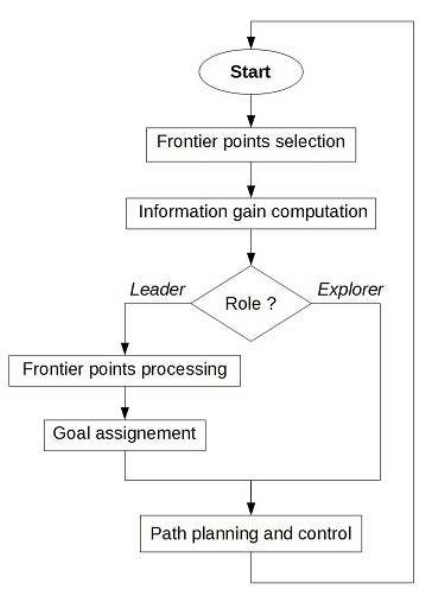
\includegraphics[scale=0.6]{assets/3_1.png}
    \caption{Proposed exploration process pipeline.}
    \label{fig:3.1}
\end{figure}
Each UAV selects the frontier points of its constructed local map during the SLAM step. Then, it computes the corresponding information gain of these points. If the UAV’s role is an \textit{explorer}, it would passively wait until receiving instructions; else, if it acts as a \textit{leader}, it would process the collected frontier points, and would assign a target to each robot in the group. Given a target, UAVs will plan a specific path to reach it.\\\\
During these steps, the map structure evolves from a projected 2D grid map obtained from the localization and mapping module, through frontier points during the frontier selection process, then candidate targets during the frontier processing step, to a final set of selected targets to reach. The evolution of the map structure is illustrated in Figure \ref{fig:3.2}. Algorithm \ref{alg:3.1} describes the main steps performed during the exploration.
\begin{algorithm}
    \caption{Exploration strategy for coordinated Multi-UAV}
    \label{alg:3.1}
    \begin{algorithmic}[1]
        \STATE From cell $\mathbf{l}_l \in \mathcal{L}$, select frontier points $\mathbf{f}_{i,j} \in \mathcal{F}$ and compute their respective information gain $\mathit{\mathbf{I}}(\mathbf{f}_{i,j})$.
        \STATE Process frontier points $\mathbf{f}_{i,j}$ to get candidate goals $\mathbf{t}_k \in \mathcal{G}$ (See Algorithm \ref{alg:3.2})
        \STATE Assign UAV$_i$ with target $k$ (See Algorithm \ref{alg:3.2}).
        \STATE Send targets to the corresponding robots.
    \end{algorithmic}
\end{algorithm}
\begin{figure}[H]
    \centering
    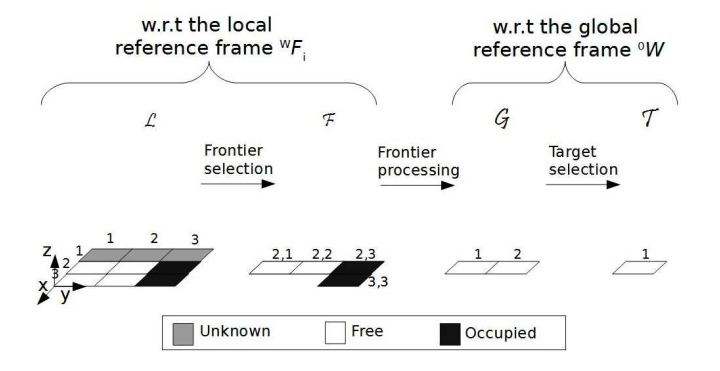
\includegraphics[scale=0.4]{assets/3_2.png}
    \caption{Map structure evolution during the exploration process: From 2D cells $\mathcal{L}$ to 2D frontier cells $\mathcal{F}$ to candidate frontier cells/points $\mathcal{G}$ (candidate targets) to 2D target cells/points $\mathcal{T}$.}
    \label{fig:3.2}
\end{figure}
\subsection{Frontier points selection}
The frontier selection process is used to define the frontiers of regions bounded by obstacles or unknown spaces (See Figure \ref{fig:3.3}).
\begin{figure}[H]
    \centering
    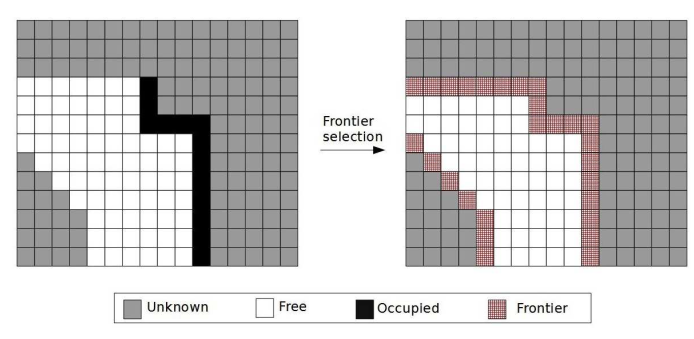
\includegraphics[scale=0.4]{assets/3_3.png}
    \caption{Frontier cells/points selection of a 2D occupancy grid map.}
    \label{fig:3.3}
\end{figure}
The frontier cells $\mathbf{f}_{i,j} \in \mathcal{F}$ are selected from the set of cells $\mathcal{L}(\mathcal{F}\subset \mathcal{L})$ such that they are either:
\begin{itemize}
    \item Free $\mathbf{l}_f$ and adjacent to unknown.
    \item Labeled as occupied $\mathbf{l}_o$ . The Occupied cells $\mathbf{l}_o$ are considered as frontier cells to be able to perform frontier processing in the next step. They could not be chosen as target and will be discarded later.
\end{itemize}
In Figure \ref{fig:3.2}, the frontier cells are: $\mathbf{l}_f(2,1)$,$\mathbf{l}_f(2,2)$ , $\mathbf{l}_f(2,3)$, and $\mathbf{l}_f(3,3)$. Thus, for a cluster $\mathcal{C}$ containing UAV$_i$ , the frontiers are:
\begin{equation} \label{eq:3.1}
    \mathcal{F}=\{\mathbf{f}_{i,1}(2,1),\mathbf{f}_{i,2}(2,2),\mathbf{f}_{i,3}(2,3),\mathbf{f}_{i,4}(3,3)\}
\end{equation}
\subsection{Information gain computation}
In frontier-based exploration approaches, only cells adjacent to unknown ones may be defined as candidate frontier points and are likely to be chosen as targets. Thereby, the information gain is associated to each of them in order to estimate the utility of reaching each frontier. This corresponding information gain can be defined in different manners depending on the mission purpose. Authors in [Burgard et al., 2005] propose to use a probability function to reduce an assigned constant value taking into account the relative distance to the UAV’s pose. This strategy is general and does not take into account the updated explored cells. The approach proposed in [Heng et al., 2015] affects, to the information gain, the number of unknown and not occluded cells in the view frustum of the target. This method depends on the real estimate of information gained when visiting the considered pose. However, it requires more computation.\\\\
In the proposed strategy, the information gain is allocated so that it defines the amount of unknown cells surrounding the target (See Figure \ref{fig:3.4}). It is a non-metric value that counts the number of cells labeled as unknown l u from the 48 cells around the frontier point.
\begin{figure}[H]
    \centering
    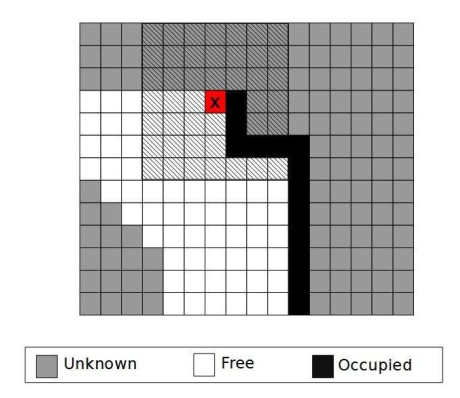
\includegraphics[scale=0.4]{assets/3_4.png}
    \caption{The information gain computation of a frontier point x (in red). The hatched cells represent the 48 surrounding cells of the frontier point \textbf{x}. The information gain of \textbf{x} is: $\mathbf{I}(x)=25$.}
    \label{fig:3.4}
\end{figure}
\subsection{Frontier points processing}
All frontier points $\mathbf{f}_{i,j} \in \mathcal{F}$ of UAV$_i$ in the cluster $\mathcal{C}$ with $i \in [1..n_c]$, are collected. Points in $\mathcal{F}$ are then processed using Algorithm \ref{alg:3.2} to get candidate frontier points considered as candidate targets $\mathbf{t}_k \in \mathcal{G}$ with $k \in [1..n_g]$ (See Figure \ref{fig:3.2})
\begin{algorithm}[H]
    \caption{Frontier processing algorithm.}
    \label{alg:3.2}
    \hspace*{\algorithmicindent} \textbf{Input:} Frontier points $\mathbf{f}_{i,j} \in \mathcal{F}$ of UAV$_i$ with $i \in [1..n_c]$. \\
    \hspace*{\algorithmicindent} \textbf{Output:} Candidate targets $\mathcal{G}$
    \begin{algorithmic}[1]
        \STATE $p_u=\cup_{i=1}^{n_c}\mathbf{f}_{i,j}$.
        \STATE $p_i=\cap_{i=1}^{n_c}\mathbf{f}_{i,j}$.
        \STATE $\mathcal{G}=p_u\setminus p_i$.
        \STATE Delete the obstacle frontier points $\mathbf{f}_{i,j}(x,y)=\mathbf{l}_o(x,y)$ from $\mathcal{G}$.
        \RETURN $\mathcal{G}$.
    \end{algorithmic}
\end{algorithm}
Figure \ref{fig:3.5} shows an example of frontier processing with two UAVs’ map to get the candidate targets. The obstacle frontier points $\mathbf{f}_{i,j}(x,y)=\mathbf{l}_o(x,y)$ – labeled as occupied – are only kept to compute the intersection of frontier points. Only the free frontier cells $\mathbf{l}_f$ can be considered as candidate target.\\\\
When using local frontier points instead of local maps, the frontier process replaces the map matching process where the aim is to clear overlapping areas. Hence, in the frontier processing step, the frontier points that belong to overlapping areas are cleared. Therefore, using frontier points allows important memory saving. To compute the frontier points that belong to the overlapped areas (Steps 1, 2 and 3 in Algorithm \ref{alg:3.2}), we propose two approaches with convex shapes and concave shapes assumptions.
\subsubsection{First approach: Convex shape map}
In this approach, map shapes are considered convex, which simplifies the intersection computation in Algorithm \ref{alg:3.3}. Figure \ref{fig:3.6} shows two examples of applying frontier processing algorithm while assuming convex shapes with two and three UAVs’ map.\\\\
This algorithm is relatively easy to apply, but results show that it does not perform well. The convex assumption leads to some false overlapped frontier points. Consequently, some unknown areas will not be visited since their corresponding points are removed and, thus, will not be assigned as a target.
\subsubsection{Second approach: Concave shape map}
In the second approach, we make the assumption of concave shapes for the UAVs’ map to compute their intersection in Algorithm \ref{alg:3.4}. Figure \ref{fig:3.7} shows two examples of applying frontier processing algorithm while assuming convex shapes with two and three UAVs’ map.
\begin{figure}[H]
    \centering
    \begin{subfigure}[H]{0.6\linewidth}
        \centering
        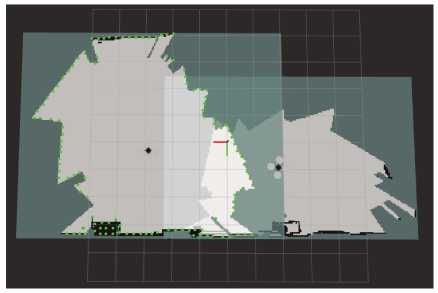
\includegraphics[width=\linewidth]{assets/3_5_a.png}
        \caption{{Frontiers $\mathbf{f}_{1,j}$ of UAV$_1$}}
        \label{fig:3.5a}
    \end{subfigure}
    \begin{subfigure}[H]{0.6\linewidth}
        \centering
        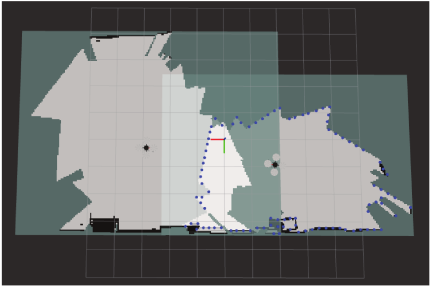
\includegraphics[width=\linewidth]{assets/3_5_b.png}
        \caption{{Frontiers $\mathbf{f}_{2,j}$ of UAV$_2$}}
        \label{fig:3.5b}
    \end{subfigure}
    \begin{subfigure}[H]{0.6\linewidth}
        \centering
        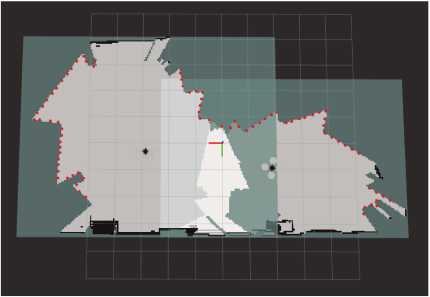
\includegraphics[width=\linewidth]{assets/3_5_c.png}
        \caption{{Candidate targets $\mathcal{G}$}}
        \label{fig:3.5c}
    \end{subfigure}
    \caption{Frontier points processing example: (a) and (b) represent the frontier points of UAV$_1$ and UAV$_2$, respectively. (c) represent the candidate targets. The process consists in removing frontier points that belong to overlapped areas, and those that are adjacent to obstacles.}
    \label{fig:3.5}
\end{figure}
\begin{algorithm}[H]
    \caption{Intersection computation algorithm with convex shapes assumption.}
    \label{alg:3.3}
    \hspace*{\algorithmicindent} \textbf{Input:} $Vect1, Vect2$ \\
    \hspace*{\algorithmicindent} \textbf{Output:} $Vect\_Final$
    \begin{algorithmic}[1]
        \FOR {$i \in Vect1$}
        \STATE $inf = 0, sup = 0$
        \FOR{ $j \in Vect2$}
        \IF {$Vect1(i).x < Vect2(i).x$}
        \STATE $inf++$;
        \ELSE
        \STATE $sup++$;
        \ENDIF
        \ENDFOR
        \IF {$inf>0$ and $sup>0$}
        \STATE $Vect\_inter.push\_back(Vect1(i))$
        \ENDIF
        \ENDFOR
        \FOR{$i \in Vect\_inter$}
        \STATE $inf=0,sup=0$;
        \FOR{$j \in Vect2$}
        \IF {$|Vect\_inter(i).x-Vect2(i).x| <0.5$}
        \STATE $inf++$;
        \ELSE
        \STATE $sup++$;
        \ENDIF
        \ENDFOR
        \IF {$inf>0$ and $sup>0$}
        \STATE $Vect\_Final.push\_back(Vect\_inter(i))$
        \ENDIF
        \ENDFOR
    \end{algorithmic}
\end{algorithm}
\begin{figure}[H]
    \centering
    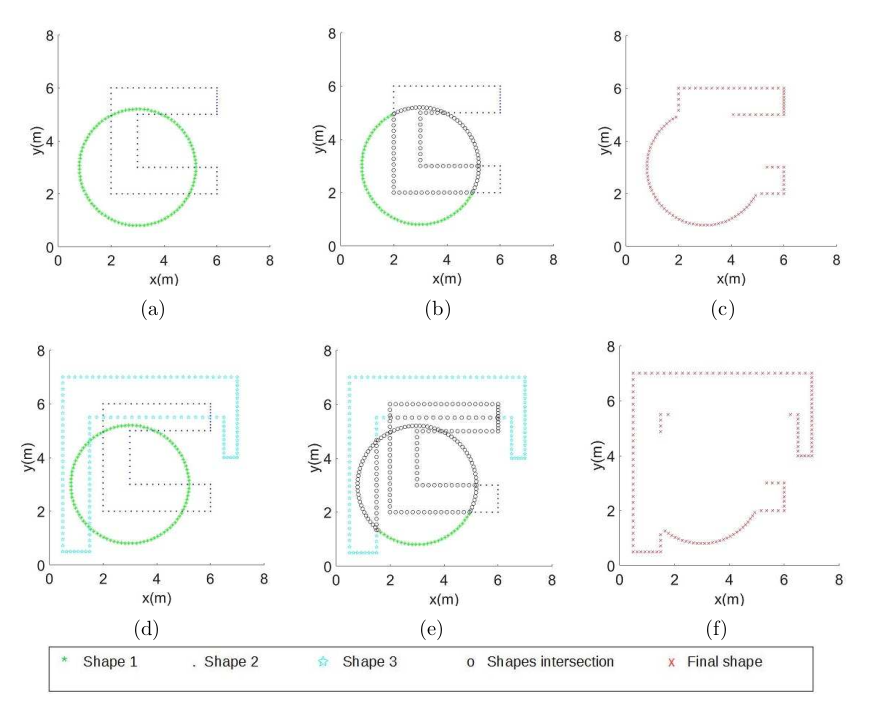
\includegraphics[scale=0.4]{assets/3_6.png}
    \caption{Frontier points processing wile assuming two convex map shapes in the first line and three in the second line. (a) and (d) represent two and three convex map shapes, respectively; (b) and (e) represent the frontier points in overlap (intersection); and (c) and (f) represent the obtained frontier points after processing (final shape).}
    \label{fig:3.6}
\end{figure}
\begin{algorithm}[H]
    \caption{Intersection computation algorithm with convex shapes assumption.}
    \label{alg:3.4}
    \hspace*{\algorithmicindent} \textbf{Input:} $Vect1, Vect2$ \\
    \hspace*{\algorithmicindent} \textbf{Output:} $Vect\_Final$
    \begin{algorithmic}[1]
        \FOR {$i \in Vect1$}
        \STATE $inf = 0, sup = 0$
        \FOR{ $j \in Vect2$}
        \IF {$Vect1(i).x < Vect2(i).x -0.5$}
        \STATE $inf++$;
        \ELSIF {$Vect1(i).x>Vect2(i).x+0.5$}
        \STATE $sup++$;
        \ELSE
        \STATE $eq++$;
        \ENDIF
        \ENDFOR
        \IF {$inf>0$ and $sup>0$ or $eq>0$}
        \STATE $Vect\_inter.push\_back(Vect1(i))$
        \ENDIF
        \ENDFOR
        \FOR{$i \in Vect\_inter$}
        \STATE $inf=0,sup=0, eq=0$;
        \FOR{$j \in Vect2$}
        \IF {$|Vect\_inter(i).y-Vect2(i).y| <0.5$}
        \IF {$Vect\_inter(i).x<Vect2(i).x-0.5$}
        \STATE $inf++$;
        \ELSIF {$Vect1(i).x>Vect2(i).x+0.5$}
        \STATE $sup++$;
        \ELSE
        \STATE $eq++$;
        \ENDIF
        \ENDIF
        \ENDFOR
        \IF {($inf>0$ and $sup>0$) or $eq>0$}
        \STATE $Vect\_Final.push\_back(Vect\_inter(i))$
        \ENDIF
        \ENDFOR
    \end{algorithmic}
\end{algorithm}
\begin{figure}[H]
    \centering
    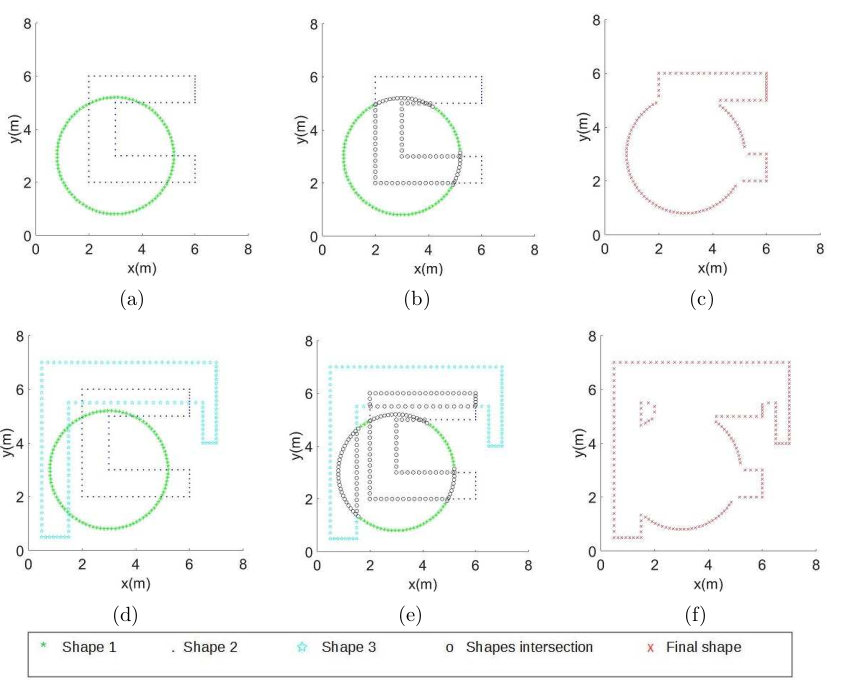
\includegraphics[scale=0.4]{assets/3_7.png}
    \caption{Frontier points processing wile assuming two concave map shapes in the first line and three in the second line. (a) and (d) represent two and three convex map shapes, respectively; (b) and (e) represent the frontier points in overlap (intersection); and (c) and (f) represent the obtained frontier points after processing (final shape).}
    \label{fig:3.7}
\end{figure}
Results show that only the frontier points within overlapping areas are removed. Even if some ambiguous frontier points are located within/inside the global shape – which can be confusing –, they are not deleted. This algorithm, assuming concave shapes, performs better than the previous one that assumes convex shapes. Hence, for the frontier processing, the shape of local maps are assumed concave.
\subsubsection{Utility function}
The proposed utility function in Eq. \ref{eq:3.2} aims to simultaneously increase the explored area rate and to reduce the distance of each UAV to its corresponding target. The function also considers the average of distances between each robot in the group and this target in order to maximize distances among robots.
\begin{equation}
    \mathbf{U}(UAV_i,t_j)=\mathbf{I}(t_j)exp(-\lambda.(dmin(\mathbf{P}_i,\mathbf{t}_j)+\frac{n_c-1}{d_{tot}})),
\end{equation}
where UAV i is the considered robot, $\mathbf{t}_j \in \mathcal{G}$ and $\mathbf{I}(\mathbf{t}_j)$ are respectively the candidate target and its corresponding information gain, $\lambda \in [0,1]$ is a trade-off parameter, $n_c$ is the number of UAVs in the cluster $\mathcal{C}$, and $d_{tot} = \sum_{k=1, k\neq i}^{n_c}(dmin(\mathbf{P}_k),\mathbf{t}_j) $ is the sum of the minimum distance from UAV$_k$'s pose $\mathbf{P}_k$ to the candidate target $j$. The proposed utility function is inspired from [Heng et al., 2015] and it has been presented in our works [Mahdoui et al., 2017, Mahdoui et al., 2018]. This function performs a trade-off between rapid exploration and a precise filling the map using a tuning parameter $\lambda$. From Figure \ref{fig:3.8}, we can notice that the larger $\lambda$, the less important the distance $d_{tot}$. Thus, a precise filling is favored over rapid exploration and vice versa.\\\\
Regarding the Multi-UAV case, the utility function is based on the average of neighbors distances. As shown in Figure \ref{fig:3.8}, with an information gain of $\mathbf{I}(\mathbf{t}_j)=25$ and three UAVs in the cluster $(n_c=3)$; an increasing distance of UAV to the target will reduce the utility function. Whereas, the larger the average distance from other UAVs w.r.t. to the target, the more the utility. So the function tends to choose the closest target to the considered UAV; but at the same time, the farthest one from the others.\\\\
In the case of a single UAV, the utility function (See Eq. \ref{fig:3.3}) tends to choose the closest target with the maximum of information gain:
\begin{equation}
    \mathbf{U}(UAV_i,\mathbf{t}_j)=\mathbf{I}(\mathbf{t}_j)exp(-\lambda.(dmin(\mathbf{P}_j,\mathbf{t}_j))),
\end{equation}
The parameter $d_{tot} = \sum_{k=1, k\neq i}^{n_c}(dmin(\mathbf{P}_k,\mathbf{t}_j)) $ represents the sum of the minimum distance between the target $\mathbf{t}_j$ and the neighbors’ poses $\mathbf{P}_k$ with $k \in [1..n_c]\setminus i$. So, if $\mathbf{t}_j$ has neighboring UAVs that are too far, the utility function will increase, so t j is more likely to be chosen.\\\\
The aim in the utility function is to maximize $d_{tot}$ . We distinguish two cases where $d_{tot}$ can be too close to zero or equal to it:
\begin{figure}[H]
    \centering
    \begin{subfigure}[H]{0.4\linewidth}
        \centering
        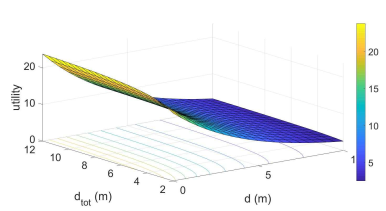
\includegraphics[width=\linewidth]{assets/3_8_a.png}
        \caption{{$\lambda=0.2$}}
        \label{fig:3.8a}
    \end{subfigure}
    \begin{subfigure}[H]{0.4\linewidth}
        \centering
        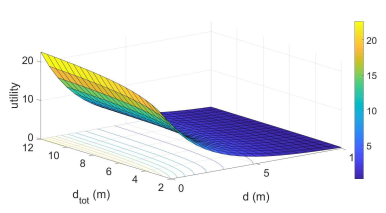
\includegraphics[width=\linewidth]{assets/3_8_b.png}
        \caption{{$\lambda=0.4$}}
        \label{fig:3.8b}
    \end{subfigure}
    \begin{subfigure}[H]{0.4\linewidth}
        \centering
        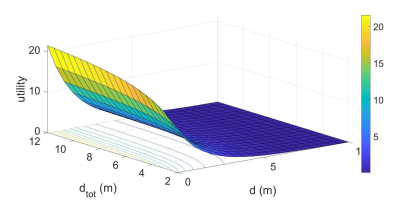
\includegraphics[width=\linewidth]{assets/3_8_c.png}
        \caption{{$\lambda=0.6$}}
        \label{fig:3.8c}
    \end{subfigure}
    \begin{subfigure}[H]{0.4\linewidth}
        \centering
        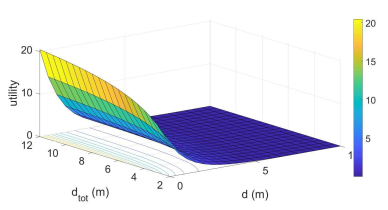
\includegraphics[width=\linewidth]{assets/3_8_d.png}
        \caption{{$\lambda=0.8$}}
        \label{fig:3.8d}
    \end{subfigure}
    \caption{{Utility function behavior: $\mathbf{I}(t_j)=25, n_c=3, d_{tot} = \sum_{k=1, k\neq i}^{n_c}(dmin(\mathbf{P}_k,\mathbf{t}_j))$. The average distance of other UAVs $d_{tot}$ has a minimum value different from zero since $n_c$ is different from zero too.}}
    \label{fig:3.8}
\end{figure}
\begin{itemize}
    \item There are no neighbors. In this case, there is one UAV in the fleet: $n_c=1$. The utility function in Eq. \ref{eq:3.3} is used.
    \item The candidate target $\mathbf{t}_j$ and the neighbors’ poses $\mathbf{P}_k$ with $k \in [1..n_c]\setminus i$ are almost confused (too close to each others). In this case $\mathbf{t}_j$ is less likely to be chosen.
\end{itemize}
Yet, this parameter $d_{tot}$ could have a high value when:
\begin{itemize}
    \item There is one UAV too far from $\mathbf{t}_j$.
    \item There are several UAVs with relatively short distance from $\mathbf{t}_j$.
\end{itemize}
So, in order to avoid these ambiguous situations, the average of $d_{tot}$ is considered by using $\frac{n_c}{d_{tot}}$.
\subsection{Goal assignment process}
In order to make appropriate UAV-to-target assignment, the utility of reaching each candidate frontier is considered. The goal assignment process is described in Algo. \ref{alg:3.5}.\\\\
For each UAV$_i$ , the utilities of reaching all the candidate targets are computed. The target $\mathbf{t}_g$ that maximizes the utility is computed and, the assignment $\theta(UAV_i,\mathbf{t}_g)$ is performed. Then, the remaining candidate targets $\mathcal{G}\setminus \mathcal{T}$ are scheduled in order to avoid to select a target too close to $\mathbf{t}_g$ , in the next iteration. Also, $\mathbf{t}_g$ is removed from $\mathcal{G}$ to prevent from assigning the same target to different robots. This assignment process is performed for the available UAVs in $\mathcal{C}$ in a sequential manner until getting all assigned targets $\mathbf{t}_g \in \mathcal{T}$ with $g \in [1..n_t]$ (See Figure \ref{fig:3.2})
\begin{algorithm}[H]
    \caption{Goal assignment algorithm.}
    \label{alg:3.5}
    \hspace*{\algorithmicindent} \textbf{Input:} {Candidate targets $\mathbf{t}_k \in \mathcal{G}, k \in [1..n_g]$ and their respective information gain $\mathbf{U}(\mathbf{t}_k)$, poses $\mathbf{P}_i$ of all robots in the considered cluster $\mathcal{C}$.}\\
    \hspace*{\algorithmicindent} \textbf{Output:} {$\theta(UAV_i,\mathbf{t}_g)$ assignment of UAV$_i$ with target $g$.}
    \begin{algorithmic}[1]
        \STATE $\mathcal{T}=\theta$
        \WHILE{no goal for UAV$_i$}
        \STATE Compute its corresponding utility of reaching each remaining candidate goal $\mathbf{U}(UAV_i,\mathbf{t}_k)$ with $\mathbf{t}_k \in \mathcal{G}\setminus \mathcal{T}$.
        \STATE $t_g=argmax_{t_k \in \mathcal{G}\setminus \mathcal{T}}(\mathbf{U}(UAV_i,\mathbf{t}_k))$.
        \STATE Schedule the information gain of the remaining candidates $\mathbf{t}_k \in \mathcal{G} \setminus \mathcal{T}$.
        \STATE $\mathcal{T}=\mathcal{T}\cup t_g$.
        \ENDWHILE
        \RETURN $\theta(UAV_i, \mathbf{t}_g)$ assignment.
    \end{algorithmic}
\end{algorithm}
\subsubsection{Stop condition}
The goal selection process is realized by each cluster/group-\textit{leader} (if $n>n-c$ ) or the Fleet- \textit{leader} (if $n=n_c$). This assignment aims to, cooperatively, distribute the robots in the environment to explore simultaneously different unknown regions. As long as candidate frontier points are still available, the \textit{leader} continues to assign targets to \textit{explorers} and they attempt to reach their assigned goals. When the \textit{leader} notices that no candidate targets are left, that means that all the environment has been explored successfully and the mission is accomplished. Thus, it has to send back to the \textit{explorers} an acknowledgment to prevent them assuming a communication loss.
\subsubsection{Loop rate}
The target assignment process is performed at each loop. The frequency of assigning targets impacts the duration and the efficiency of the mission. In a distributed approach, as soon as the UAV reaches its current target, it selects a new one without consulting the others. In a centralized approach, the first UAV to reach its current target has to wait until the others reach their respective targets. This can be a problem as soon as one of them fails or leaves the mission. Another possibility is to begin to assign targets once one UAV reaches its target. But this may generate incomplete tasks. In the proposed strategy, the frequency of assignment or loop rate $r$ is predefined depending on the average of time to reach a target (See Eq. \ref{eq:3.4}).
\begin{equation} \label{eq:3.4}
    r \in [\frac{s}{v_{i,max}},\frac{s}{v_{i,min}}]
\end{equation}
where $s$ is the maximum sensor range and $v_i$ is the UAV's velocity.
\subsubsection{Scheduling the information gain}
The information gain of each remaining candidate target $\mathbf{I}(\mathbf{t}_k)_{t-1}$ at time $t-1$ with $\mathbf{t}_k \in \mathcal{G} \setminus \{t_g\}$, that belongs to the threshold range $[r_{min} , r_{max} ]$, is scheduled at time $t$ depending on its distance w.r.t. the target $t_g$ , using Eq. \ref{eq:3.5}. Figure \ref{fig:3.9} represents an example of the function shape used to schedule the information gain. The example shows a Gaussian function with an amplitude that corresponds to the information gain maximum value; a center that corresponds to the target position $(\mathbf{t}_g(x), \mathbf{t}_g(y))$; and $\sigma_x$ and $\sigma_y$ that spread the blob in $x$ and $y$ axis, respectively.
\begin{figure}[H]
    \centering
    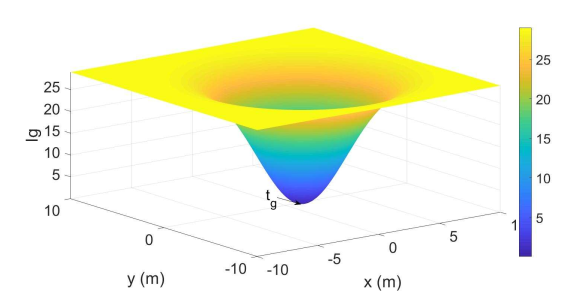
\includegraphics[scale=0.6]{assets/3_9.png}
    \caption{Example of the shape function to schedule the information gain($\mathbf{I}(\mathbf{t}_k)_{t-1}=29,(\mathbf{t}_g(x),\mathbf{t}_g(y))=(1.25,-0.275), \sigma_x=\sigma_y=3$).}
    \label{fig:3.9}
\end{figure}
\begin{equation}\label{eq:3.5}
    \mathbf{I}(\mathbf{t}_k)_t=\mathbf{I}(\mathbf{t}_k)_{t-1}(1-exp(-(\frac{(\mathbf{t}_k(x)-\mathbf{t}_g(x))^2}{2.\sigma_x^2}+\frac{(\mathbf{t}_k(y)-\mathbf{t}_g(y))^2}{2.\sigma_y^2}))),
\end{equation}
where $\mathbf{t}_k(x)$ and $\mathbf{t}_k(y)$ are the remaining candidate target coordinates; $\mathbf{t}_g(x)$ and $\mathbf{t}_g(y)$ are the target coordinates; and $\sigma_x$ and $\sigma_y$ are the spreads of the blob. The smaller the distance of the frontier point $\mathbf{t}_k$ w.r.t. the target $\mathbf{t}_g$, the smaller the information gain. When reducing the information gain, the candidate targets are less likely to be chosen and thus, robots ensure a certain distance among their future targets.
\subsection{Path planning and control}
As explained in Section 5.2 of Chapter 1, UAVs are assumed to navigate in a simplified 2D environment with a fixed $z$ value. Block \textbf{6} in Figure 1.6 is responsible for planning a path to the selected target and attempting to reach it. These tasks are ensured by the \textit{move} base\footnote{Source: \url{http://wiki.ros.org/move_base}} package.\\\\
For the navigation task, each UAV maintains a local and a global planner along with a local and a global costmap, respectively. The costmap is a 2D cell grid $\mathcal{L}$ with additional inflation that consists in propagating cost values out from occupied cells and decreasing them with distance. The global costmap has the size of the UAV’s map whereas, the local costmap has a fixed size moving window. Given a starting point – the current pose – and an endpoint – the assigned target – in the global costmap, the global planner produces a plan using a navigation function computed with Dijkstra algorithm [Dijkstra, 1959]. It consists in following the adjacent free cells until reaching the goal. Then taking into account the local costmap, the local planner generates velocity commands for the UAV’s mobile base. A recovery rotational behavior is also performed when needed in order to clear the robot’s field of view.\\\\
The target assigned by the \textit{leader} is ensured to belong to an unknown area using the exploration strategy. The trajectory planning process is performed locally on each robot. And since the UAVs do not exchange their local maps nor fuse them, they are likely to revisit already explored areas while following the planned path. To minimize these overlapped regions during navigation, a priority is given to frontier points $\mathbf{f}_{i,j}$ to be a target for UAV$_i$ over UAV$_k$ with $k \neq i$. This helps the UAV to maintain the same direction during exploration. The \textit{move} base package is a 2D navigation stack. However, to avoid drifting on the $z$ axis, a control command is added to keep a static $z$ altitude (See Figure \ref{fig:3.10}).
\begin{figure}[H]
    \centering
    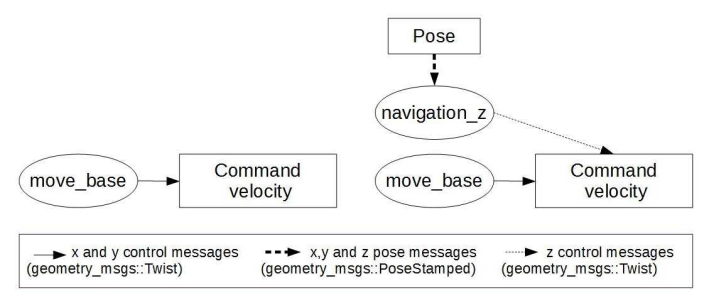
\includegraphics[scale=0.4]{assets/3_10.png}
    \caption{From 2D (left) to 3D (right) navigation stack. The \textit{navigation} z is a ROS process developed to provide a control command on the z axis.}
    \label{fig:3.10}
\end{figure}
\section{Result and discussions}
Simulations have been performed to evaluate the proposed exploration strategy. Additional tests while using relative localization have been done to measure the system performances. The simulations are performed using Robot Operating System (ROS) running on a 2.60GHz i7 Linux machine. For the quad-rotor simulation, the AR-drone model\footnote{Source: \url{http://wiki.ros.org/ardrone_autonomy}} equipped with an RGB-D camera in a forward-looking configuration, is used. A bounded unknown environment is generated using \textit{Gazebo} simulator. The number of robots used for evaluation is limited to three, however, the proposed system architecture is not constrained to a fixed number of robots.
\subsection{Parameters tuning}
For an effective evaluation of the exploration strategy, we run some tests to set the most adequate parameters configuration.
\subsubsection{Trade-off parameter $\lambda$}
The utility function (See Eq. \ref{eq:3.2}) used in the exploration strategy can be tuned, using a trade off parameter $\lambda$, between fast exploration and filling in details the map.\\\\
Figure \ref{fig:3.11} shows different runs while varying this parameter. By increasing $\lambda$, the information gained when reaching the goal is favored over the distance and thus, the cost to it, and vice versa. So, when $\lambda$ is small, the traveled distance is small and so the exploration time. Though, some times during the mission, high values of $\lambda$ are noticed to reach higher exploration rate than smaller ones.
\begin{figure}[H]
    \centering
    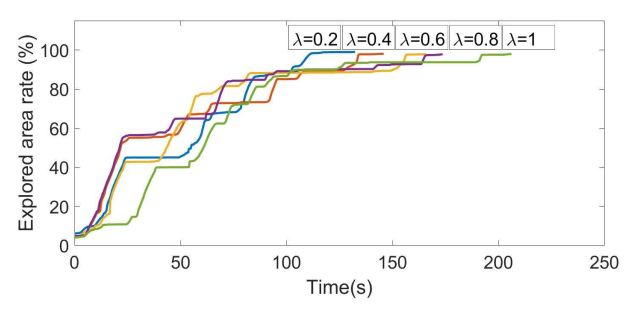
\includegraphics[scale=0.5]{assets/3_11.png}
    \caption{The impact of varying the trade off parameter $\lambda$ over exploration itme.}
    \label{fig:3.11}
\end{figure}
\subsubsection{Loop rate $r$}
The frequency or loop rate $r$ of target assignment may also affect exploration time performance. The values of $r$ vary to take into account the robot velocity $\mathbf{v}_i$ and the sensor’s maximum range $s$. The impact of varying the loop rate is evaluated in Figure \ref{fig:3.12}.
\begin{figure}[H]
    \centering
    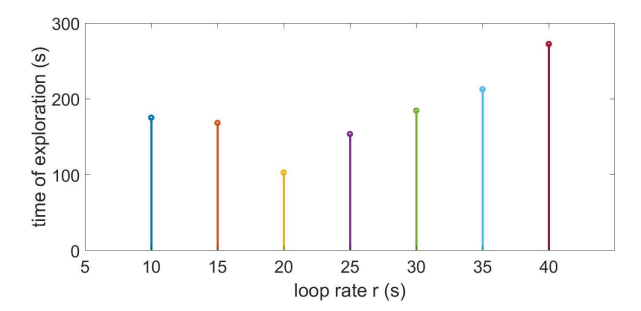
\includegraphics[scale=0.5]{assets/3_12.png}
    \caption{Exploration time while varying the loop rate $r$.}
    \label{fig:3.12}
\end{figure}
Given a robot velocity $\mathbf{v}_i=\{0.1,0.3\}m.s^{-1}$ and a maximum sensor range $s=4m$, the loop rate variates in $r \in [10,40]$. This parameter should not be too small to allow the robot to reach its target; nor too big to prevent long waiting times for the next goal assignment.
\subsubsection{Common parameters}
Depending on results in Figure \ref{fig:3.11} and Figure \ref{fig:3.12}, respectively, $\lambda$ is set to $0.2$ and $r$ to $20s$ in order to maximize the explored area rate while minimizing the mission time. The simulation parameters are summarized in Table \ref{tab:3.1}.
\begin{table}[H]
    \centering
    \caption{Common parameters.}
    \label{tab:3.1}
    \begin{tabular}{|l|l|}\hline
        \makebox[5em]{\textbf{Parameter}}                  & \makebox[5em]{\textbf{Value}}
        \\\hline
        RGB-D horizental FoV                               & $\pi/ 3$                      \\\hline
        Trade-off parameter $\lambda$                      & 0.2                           \\\hline
        RGB-D maximum range $s (m)$                        & 4                             \\\hline
        Min distance among frontiers $d (m)$               & 0.3                           \\\hline
        Occupancy grid resolution $(m)$                    & 0.05                          \\\hline
        Range to schedule the $\lg[\sigma_x,\sigma_y] (m)$ & $[3,3]$                       \\\hline
        Loop rate $l (s)$                                  & 20                            \\\hline
        Enviroment dimension $(m^2)$                       & $8 \times 8$                  \\\hline
        Linear velocity $v_i (m.s^{-1})$                   & $[0.1,0.3]$                   \\\hline
        Angular velocity $w_i (rad.s^{-1})$                & $[0.1,0.3]$                   \\\hline
    \end{tabular}
\end{table}
\subsection{Exploration strategy performances}
The proposed exploration strategy has been evaluated in terms of distribution of the robots in the environment, overlap rate, exploration time, and total traveled distance by each robot.
\subsubsection{Maps evolution during the mission}
While reaching their respective assigned goals, each robot is in charge of creating a detailed grid map of the visited area in order to get a global map of the environment. Figure \ref{fig:3.13} illustrates the growth of the reconstructed 3D occupancy grid map at different times during the mission. Note that to reach $99\%$ of coverage, a lot of time is spent.\\\\
Figure \ref{fig:3.14} shows the evolution of the respective projected 2D local grid map of two robots during a cooperative exploration mission. The global projected 2D grid map is also created and represented for evaluation (the occupancy grid matching process introduced in Algorithm 2.1 in Chapter 2 is used). The robots’ initial positions are $(1,0,0)$ for UAV$_1$ and $(1,-3,0)$ for UAV$_2$. Despite a relatively close initial position, the proposed strategy effectively spreads the robots so that UAV$_1$ is in charge of the left side of the environment and UAV$_2$ of the right one.
\subsubsection{Frontier points evolution during the mission}
The target is chosen from the candidate frontier points that define the edges of an environment not previously explored. These candidates are selected from the final frontier points of each UAV in the fleet (See Figure \ref{fig:3.15}). During the exploration mission, the local map size increases, which leads to an increasing number of local frontier points. At the beginning of the exploration, the number of candidate frontier points increases, but as soon as the exploration evolves in time, their number decreases. At the end of the mission, when all the environment is explored, no candidate frontier points should be left.
\subsubsection{UAV's trajectories during the mission}
Figure \ref{fig:3.16} shows the explored map with the trajectories using one, two and three UAVs. The UAVs try to explore the full environment while avoiding already explored areas. In a cooperative way, each UAV is in charge of visiting an area by reaching a target that belongs to a non-explored environment. These targets are assigned by the \textit{Leader} which, even if the initial poses of the UAVs are relatively close, effectively spreads them into unknown areas. The global map is composed of the superposition of all UAVs’ local maps.
\begin{figure}[H]
    \centering
    \begin{subfigure}[H]{0.3\linewidth}
        \centering
        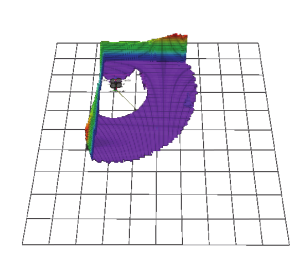
\includegraphics[width=\linewidth]{assets/3_13_a.png}
        \caption{{$3\%$ rate $(5s).$}}
        \label{fig:3.13a}
    \end{subfigure}
    \begin{subfigure}[H]{0.3\linewidth}
        \centering
        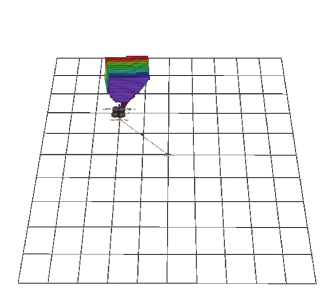
\includegraphics[width=\linewidth]{assets/3_13_b.png}
        \caption{{$20\%$ rate $(28s).$}}
        \label{fig:3.13b}
    \end{subfigure}
    \begin{subfigure}[H]{0.3\linewidth}
        \centering
        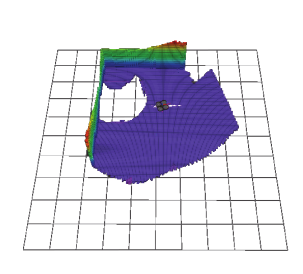
\includegraphics[width=\linewidth]{assets/3_13_c.png}
        \caption{{$31\%$ rate $(50s).$}}
        \label{fig:3.13c}
    \end{subfigure}
    \begin{subfigure}[H]{0.3\linewidth}
        \centering
        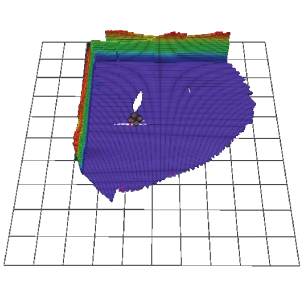
\includegraphics[width=\linewidth]{assets/3_13_d.png}
        \caption{{$40\%$ rate $(69s).$}}
        \label{fig:3.13d}
    \end{subfigure}
    \begin{subfigure}[H]{0.3\linewidth}
        \centering
        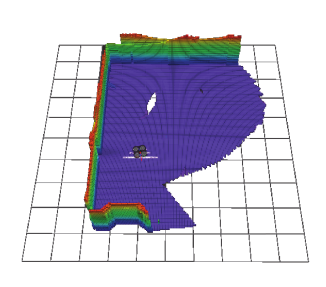
\includegraphics[width=\linewidth]{assets/3_13_e.png}
        \caption{{$50\%$ rate $(75s).$}}
        \label{fig:3.13e}
    \end{subfigure}
    \begin{subfigure}[H]{0.3\linewidth}
        \centering
        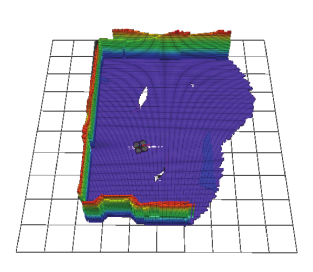
\includegraphics[width=\linewidth]{assets/3_13_f.png}
        \caption{{$60\%$ rate $(83s).$}}
        \label{fig:3.13f}
    \end{subfigure}
    \begin{subfigure}[H]{0.3\linewidth}
        \centering
        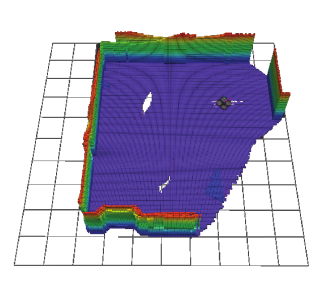
\includegraphics[width=\linewidth]{assets/3_13_g.png}
        \caption{{$70\%$ rate $(98s).$}}
        \label{fig:3.13g}
    \end{subfigure}
    \begin{subfigure}[H]{0.3\linewidth}
        \centering
        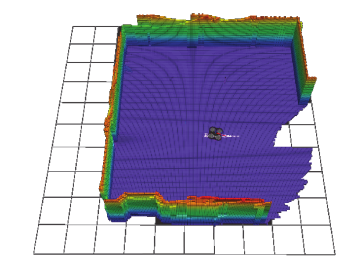
\includegraphics[width=\linewidth]{assets/3_13_h.png}
        \caption{{$81\%$ rate $(127s).$}}
        \label{fig:3.13h}
    \end{subfigure}
    \begin{subfigure}[H]{0.3\linewidth}
        \centering
        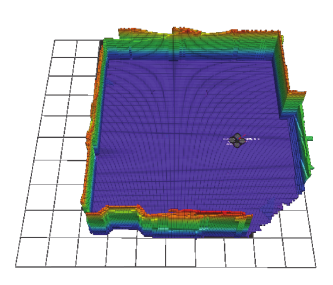
\includegraphics[width=\linewidth]{assets/3_13_i.png}
        \caption{{$90\%$ rate $(133s).$}}
        \label{fig:3.13i}
    \end{subfigure}
    \begin{subfigure}[H]{0.3\linewidth}
        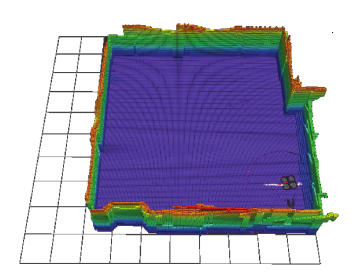
\includegraphics[width=\linewidth]{assets/3_13_j.png}
        \caption{{$99\%$ rate $(202s).$}}
        \label{fig:3.13j}
    \end{subfigure}
    \caption{Ratio of explored space during time for one UAV.}
    \label{fig:3.13}
\end{figure}
\begin{figure}[H]
    \centering
    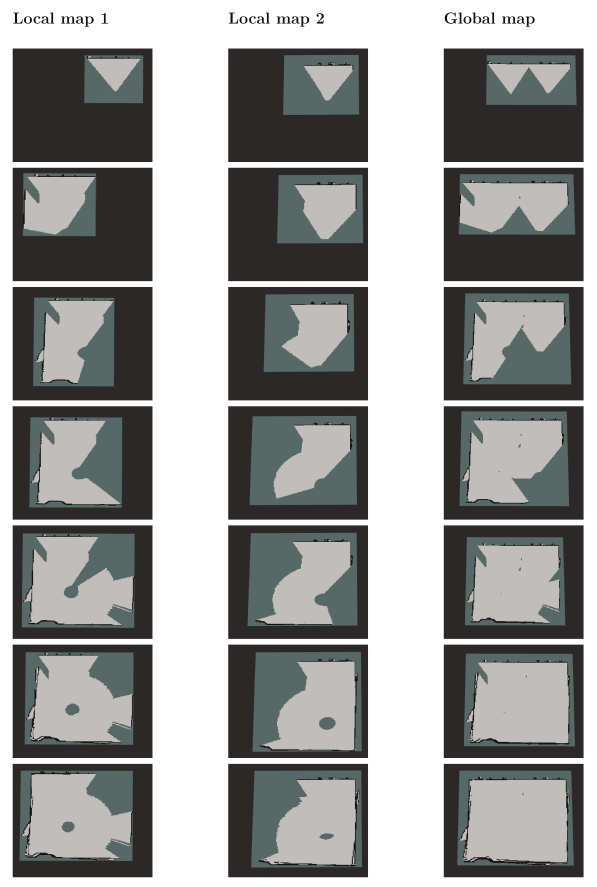
\includegraphics[scale=0.5]{assets/3_14.png}
    \caption{Coordinated exploration using two robots. Columns 1, 2 and 3 show the evolution of the local map of the UAV$_1$, the UAV$_2$ and the global map over time, respectively.}
    \label{fig:3.14}
\end{figure}
\begin{figure}[H]
    \centering
    \begin{subfigure}[H]{0.7\linewidth}
        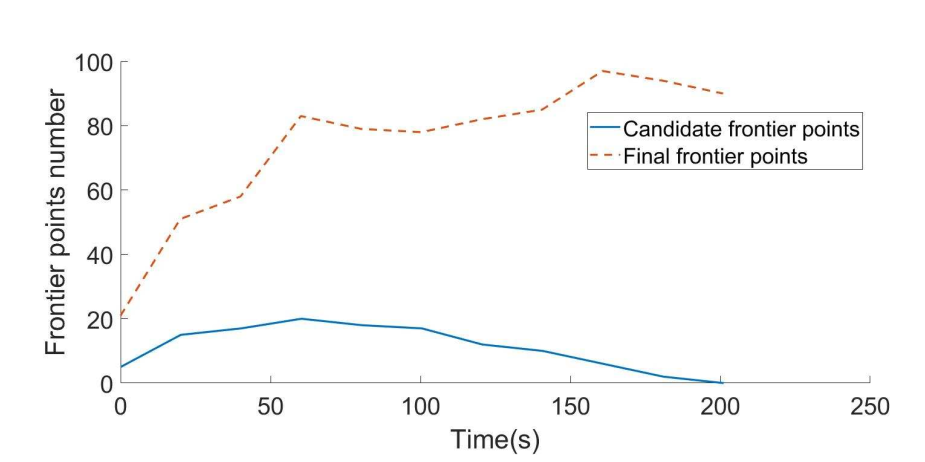
\includegraphics[width=\linewidth]{assets/3_15_a.png}
        \caption{{One UAV.}}
        \label{fig:3.15a}
    \end{subfigure}
    \begin{subfigure}[H]{0.7\linewidth}
        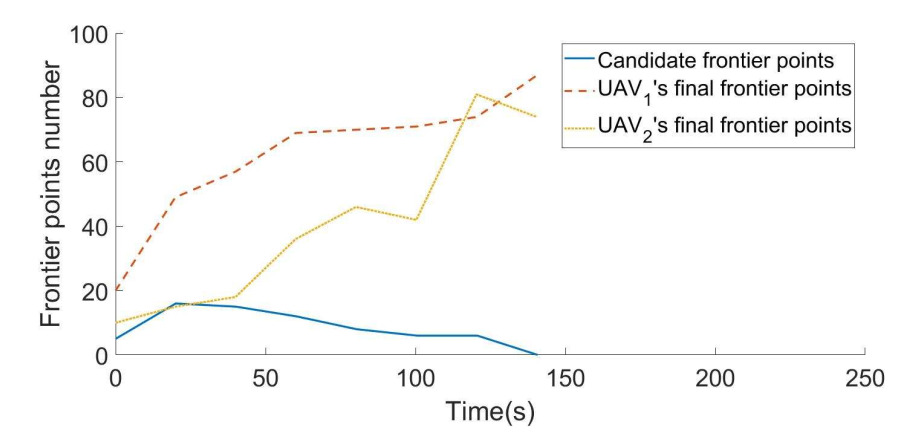
\includegraphics[width=\linewidth]{assets/3_15_b.png}
        \caption{{Two cooperative UAVs.}}
        \label{fig:3.15b}
    \end{subfigure}
    \begin{subfigure}[H]{0.7\linewidth}
        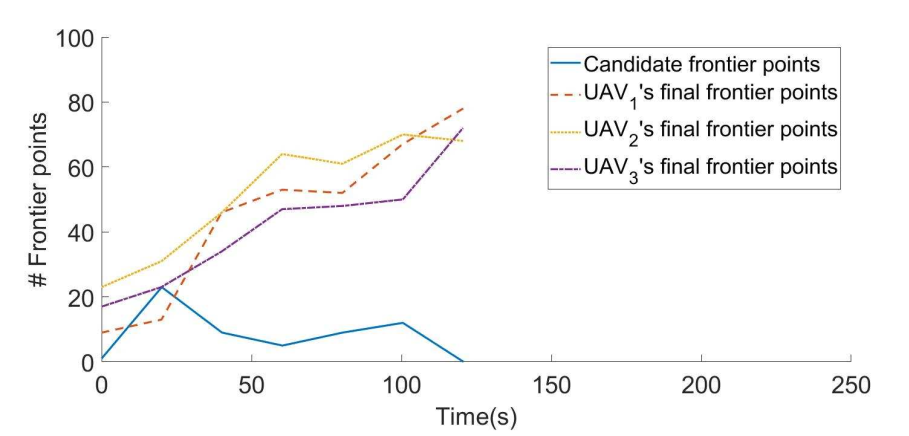
\includegraphics[width=\linewidth]{assets/3_15_c.png}
        \caption{{Three cooperative UAVs}}
        \label{fig:3.15c}
    \end{subfigure}
    \caption{The evolution of candidate and final frontier points numbers during cooperative exploration.}
    \label{fig:3.15}
\end{figure}
\begin{figure}[H]
    \centering
    \begin{subfigure}[H]{0.5\linewidth}
        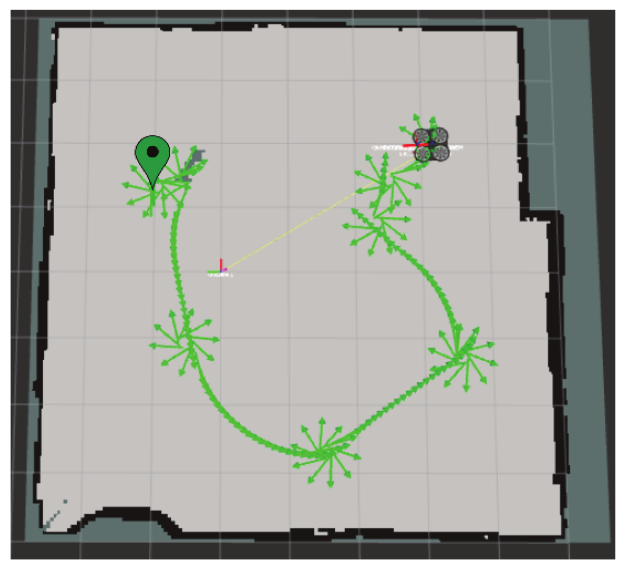
\includegraphics[width=\linewidth]{assets/3_16_a.png}
        \caption{{One UAV.}}
        \label{fig:3.16a}
    \end{subfigure}
    \begin{subfigure}[H]{0.5\linewidth}
        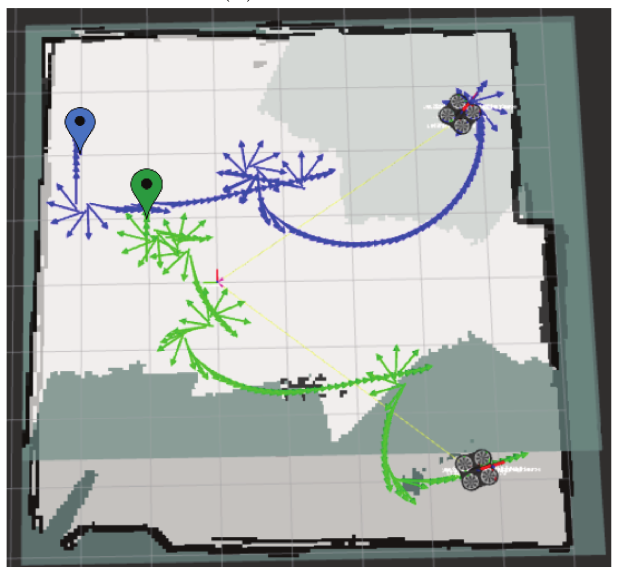
\includegraphics[width=\linewidth]{assets/3_16_b.png}
        \caption{{Two cooperative UAVs.}}
        \label{fig:3.16b}
    \end{subfigure}
    \begin{subfigure}[H]{0.5\linewidth}
        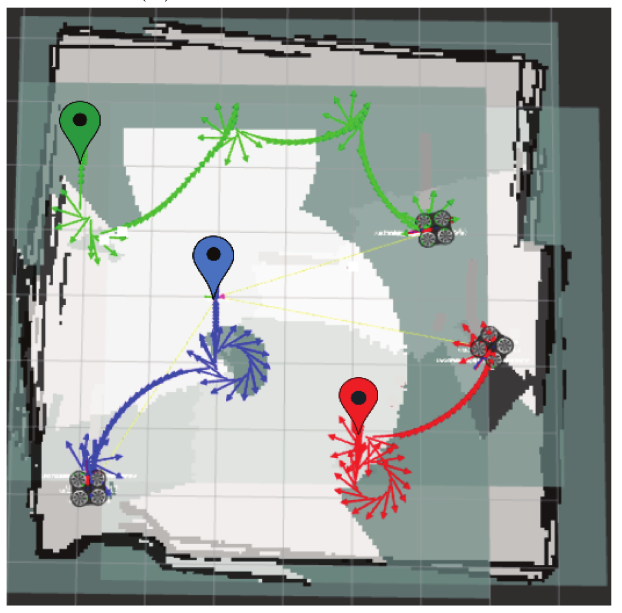
\includegraphics[width=\linewidth]{assets/3_16_c.png}
        \caption{{Three cooperative UAVs}}
        \label{fig:3.16c}
    \end{subfigure}
    \caption{Projected 2D map in a coordinated exploration with a team of one, two and three UAVs. Green, blue and red markers and arrows define, respectively, the initial position and the trajectory of UAV1, UAV2 and UAV3.}
    \label{fig:3.16}
\end{figure}
\subsubsection{Goal assignment evaluation: Distribution of the robots in the environment}
The goal assignment process is performed according to the algorithm described in Section 3.6. Nevertheless, after assigning a target to the first robot in the list, the same target or another one close to it may be assigned to the second robot in the list. To overcome these issues, the information gains of the remaining candidate targets are scheduled. This allows to discard an already assigned target and keep a certain distance between the new target and the previous one assigned.\\\\
Suppose that a target is assigned to the first robot in the cluster list. Figure \ref{fig:3.17} shows the goal selected for the second robot when a sequential assignment is performed:
\begin{itemize}
    \item Without further frontier points processing (See Figure \ref{fig:3.17b}). Consequently, the same target is assigned to two different robots.
    \item While removing the assigned target from the remaining candidate frontier points (See Figure \ref{fig:3.17c}). Consequently, the second target is relatively close to the first one assigned.
    \item While scheduling the information gain after each target assignment (See Figure \ref{fig:3.17d}). Consequently, the assigned targets are spaced out into the environment. The information gain is scheduled following Eq. \ref{eq:3.5}. The information gain value increases with distance to the candidate target $\mathbf{t}_g$.
\end{itemize}
The goal assignment process may sometimes be not optimal since it depends on the robots’ order in the list. For example, suppose that robots UAV$_i$ and UAV$_j$ have the same best target assignment t k such that it offers the maximum utility over candidate frontier points where Eq.\ref{eq:3.6} and Eq. \ref{eq:3.7} are verified.
\begin{equation}\label{eq:3.6}
    \mathbf{t}_k=argmax_{t_m}\mathbf{U}(UAV_i,\mathbf{t}_m)
\end{equation}
with $\mathbf{t}_m \in \mathcal{G}$.
\begin{equation}\label{eq:3.7}
    \mathbf{t}_k=argmax_{t_n}\mathbf{U}(UAV_j, \mathbf{t}_n)
\end{equation}
with $\mathbf{t}_n \in \mathcal{G}$.\\
UAV$_i$ have another candidate frontier point $\mathbf{t}_l$ with:
\begin{equation}\label{eq:3.8}
    \mathbf{\mathit{U}}(UAV_i, \mathbf{t}_k) > \mathbf{\mathit{U}}(UAV_i,\mathbf{t}_l) > \mathbf{\mathit{U}}(UAV_j, \mathbf{t}_k)
\end{equation}

\begin{figure}[H]
    \centering
    \begin{subfigure}[H]{0.6\linewidth}
        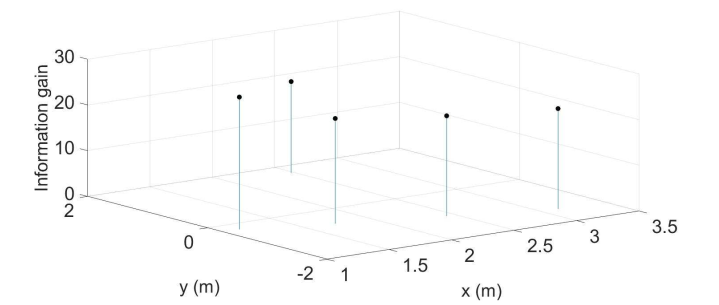
\includegraphics[width=\linewidth]{assets/3_17_a.png}
        \caption{{Candidate targets.}}
        \label{fig:3.17a}
    \end{subfigure}
    \begin{subfigure}[H]{0.6\linewidth}
        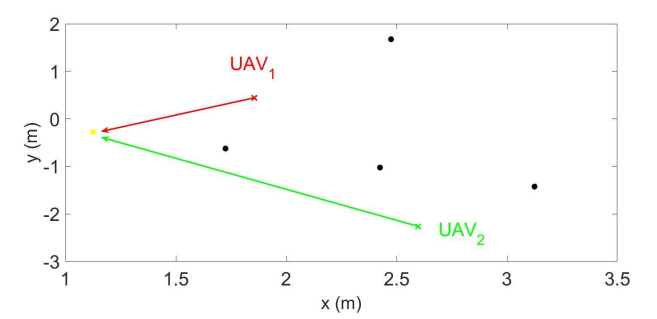
\includegraphics[width=\linewidth]{assets/3_17_b.png}
        \caption{{Case 1.}}
        \label{fig:3.17b}
    \end{subfigure}
    \begin{subfigure}[H]{0.6\linewidth}
        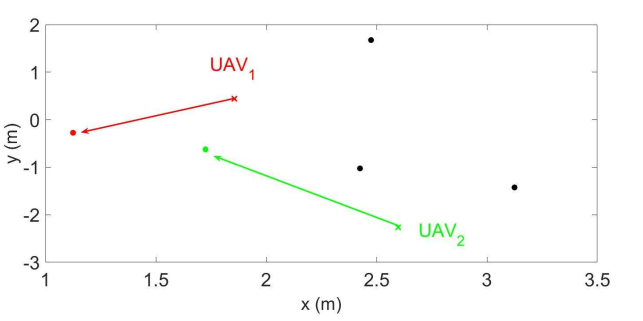
\includegraphics[width=\linewidth]{assets/3_17_c.png}
        \caption{{Case 2.}}
        \label{fig:3.17c}
    \end{subfigure}
    \begin{subfigure}[H]{0.6\linewidth}
        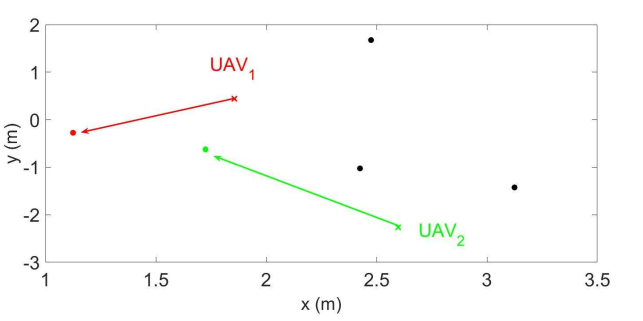
\includegraphics[width=\linewidth]{assets/3_17_c.png}
        \caption{{Case 3.}}
        \label{fig:3.17d}
    \end{subfigure}
    \caption{Goal assignment: After assigning a target to UAV$_1$ , a target is assigned in a sequential manner to UAV$_2$ . (a) represents the candidate frontier points with their respective information gain. (b), (c), and (d) represent, respectively, the targets assignment when: No further process is performed for the remaining candidate targets; UAV$_1$ ’s target is removed from the remaining candidate targets and; the information gain of the remained candidate targets are scheduled.}
    \label{fig:3.17}
\end{figure}
So the optimal solution would be to assign $\mathbf{t}_l$ to UAV$_i$ and $\mathbf{t}_k$ to UAV$_j$ . But, if UAV$_i$ is the first in the list, $\mathbf{t}_k$ is assigned to it and another candidate frontier point with less utility than $\mathbf{t}_k$, is assigned to UAV$_j$. Thus, the solution with sequential goal assignment is not always optimal.\\\\
To overcome this problem, all the numbers of possible combination $\frac{n_g!}{n_g!(n_g-n_c)!}$ with $n_g$ the number of candidate targets and $n_c$ the number of robots, need to be considered. This increases considerably the computation time by increasing the number of robots. Therefore, in the proposed algorithm, sequential assignment is favored over computing all possible permutations.
\subsubsection{Explored space rate evaluation}
This evaluation aims at quantifying the amount of explored spaces during the mission. Figure \ref{fig:3.18} shows the explored space rate performed by each UAV in the fleet. The more UAVs in the environment, the less the exploration rate demanded by each one. A robot has no need to continue exploring an area if it has already been explored by another one. Thus, the mission time is considerably reduced.
\subsubsection{Overlap rate evaluation}
The use of an effective goal assignment process should limit the generated overlap. In Figure \ref{fig:3.19}, the time evolution of overlap is evaluated using two cooperative robots. The overlap undergoes a significant increase at the end of the exploration to reach $33\%$. This is explained by the closeness of the local maps at the end of the mission to precisely fill the global grid map.
\begin{figure}[H]
    \centering
    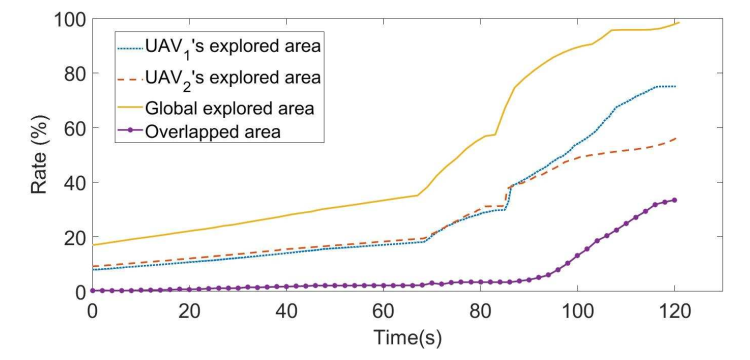
\includegraphics[scale=0.4]{assets/3_19.png}
    \caption{Explored and overlapped area rate using two cooperative UAVs.}
    \label{fig:3.19}
\end{figure}
\subsubsection{Traveled distance evaluation}
To effectively evaluate the exploration strategy performance in terms of distance traveled by each UAV, different runs with one, two and three UAVs have been conducted where explored area rate reaches almost $99\%$. Figure \ref{fig:3.20} shows the distance traveled by each UAV in the fleet during the mission.
\begin{figure}[H]
    \centering
    \begin{subfigure}[H]{0.7\linewidth}
        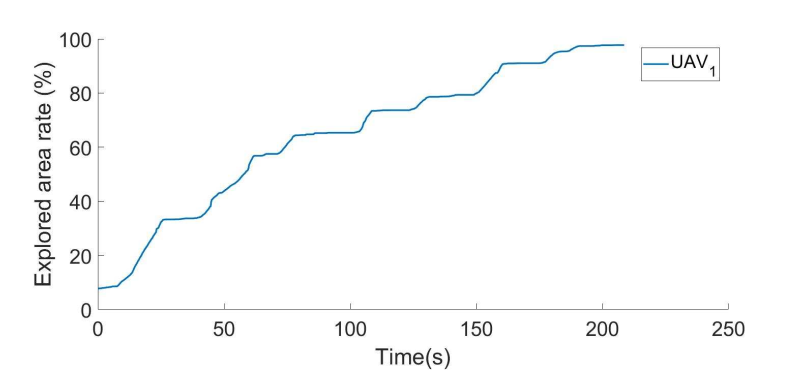
\includegraphics[width=\linewidth]{assets/3_18_a.png}
        \caption{{One UAV.}}
        \label{fig:3.18a}
    \end{subfigure}
    \begin{subfigure}[H]{0.7\linewidth}
        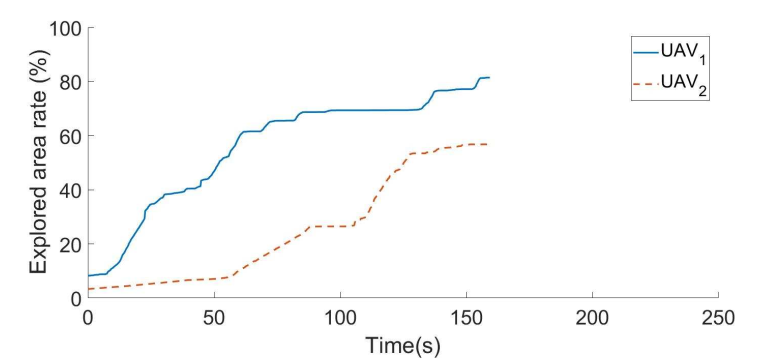
\includegraphics[width=\linewidth]{assets/3_18_b.png}
        \caption{{Two cooperative UAVs.}}
        \label{fig:3.18b}
    \end{subfigure}
    \begin{subfigure}[H]{0.7\linewidth}
        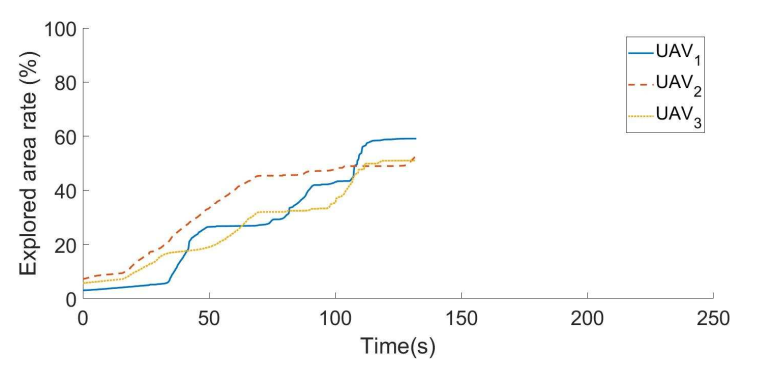
\includegraphics[width=\linewidth]{assets/3_18_c.png}
        \caption{{Three cooperative UAVs}}
        \label{fig:3.18c}
    \end{subfigure}
    \caption{Explored space rate with one, two and three UAVs.}
    \label{fig:3.18}
\end{figure}
\begin{figure}[H]
    \centering
    \begin{subfigure}[H]{0.7\linewidth}
        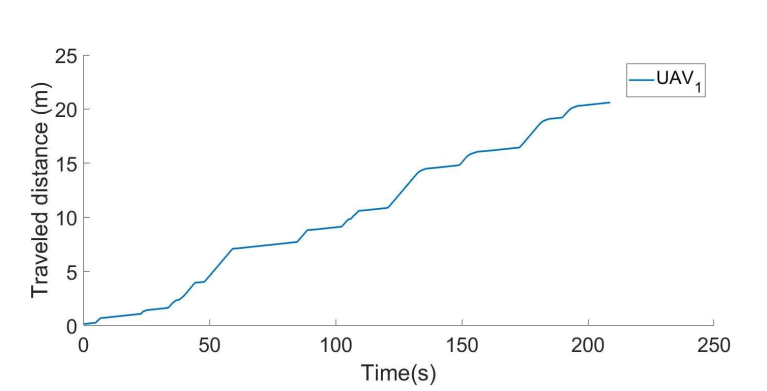
\includegraphics[width=\linewidth]{assets/3_20_a.png}
        \caption{{One UAV.}}
        \label{fig:3.20a}
    \end{subfigure}
    \begin{subfigure}[H]{0.7\linewidth}
        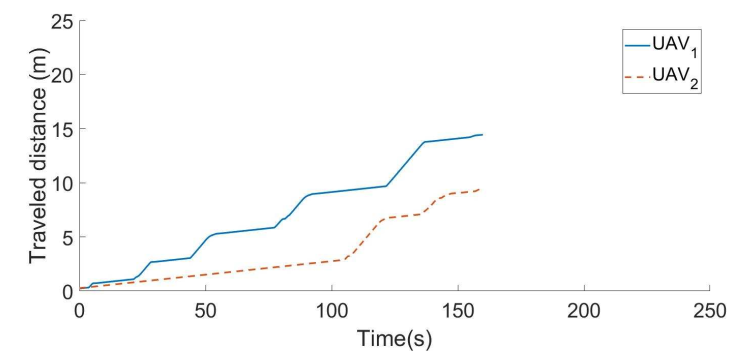
\includegraphics[width=\linewidth]{assets/3_20_b.png}
        \caption{{Two cooperative UAVs.}}
        \label{fig:3.20b}
    \end{subfigure}
    \begin{subfigure}[H]{0.7\linewidth}
        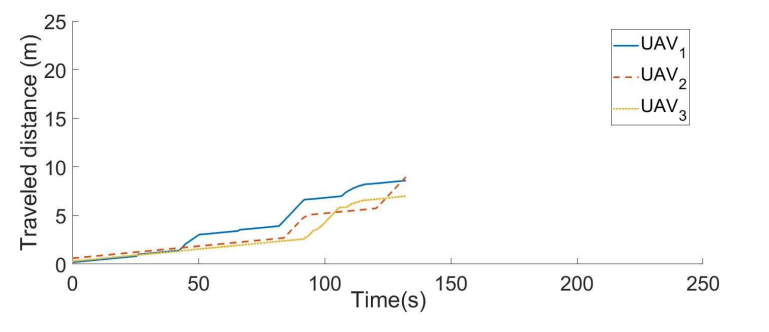
\includegraphics[width=\linewidth]{assets/3_20_c.png}
        \caption{{Three cooperative UAVs}}
        \label{fig:3.20c}
    \end{subfigure}
    \caption{Traveled distance by each UAV with one, two and three cooperative UAVs.}
    \label{fig:3.20}
\end{figure}
The distances traveled by each UAV using one, two and three UAVs in the fleet are compared in Figure \ref{fig:3.21}. This distance decreases with the number of UAVs. The average distance traveled by each UAV is reduced by $55\%$ for 2 UAVs and by $62\%$ for 3 UAVs. The error of the traveled distance is slightly reduced from one to two and three UAVs.
\begin{figure}[H]
    \centering
    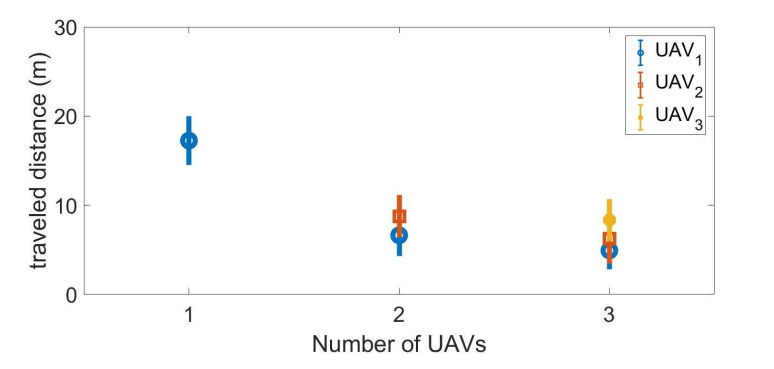
\includegraphics[scale=0.4]{assets/3_21.png}
    \caption{Traveled distance evaluation.}
    \label{fig:3.21}
\end{figure}
\subsubsection{Exploration time evaluation}
For the exploration time evaluation, different runs have been performed using 1, 2 and 3 UAVs. Figure \ref{fig:3.22} shows that the average of exploration time decreases when the number of robots in the fleet increases. The computed error decreases as well. The time is reduced by $25\%$ for 2 UAVs and by $30\%$ for 3 UAVs. The exploration time and distance are not divided by 2 or 3 when multiplying by 2 or 3 the number of robots, respectively. During these simulations, the robots’ initial positions are: $(1,0,0)$ for one UAV; $(1,0,0)$ and $(1,-3,0)$ for two UAVs; and $(1,1,0)$, $(1,-1,0)$ and $(1,-3,0)$ for three UAVs.
\begin{figure}[H]
    \centering
    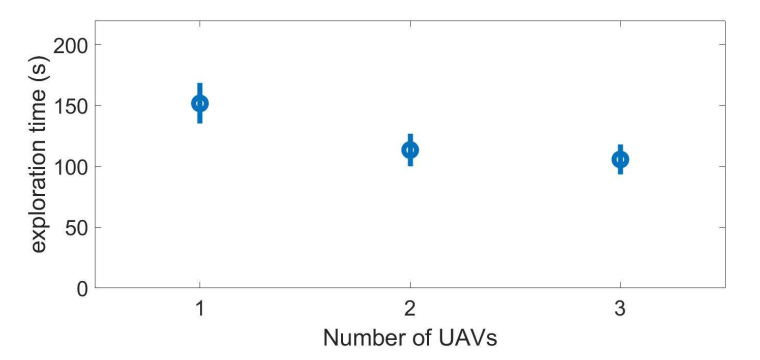
\includegraphics[scale=0.4]{assets/3_22.png}
    \caption{Average exploration time.}
    \label{fig:3.22}
\end{figure}
The results presented in Section 4.2 were evaluated without a relative localization. So, for a more challenging realistic scenario, runs with relative localization algorithm have been performed to evaluate system performances using SLAM.
\subsection{Exploration mission using relative localization algorithm}
Toward a more realistic scenario, the ORB-SLAM2 approach (introduced in Section 5 of Chapter 2) has been implemented to perform relative localization (See Figure \ref{fig:3.23}).
\begin{figure}[H]
    \centering
    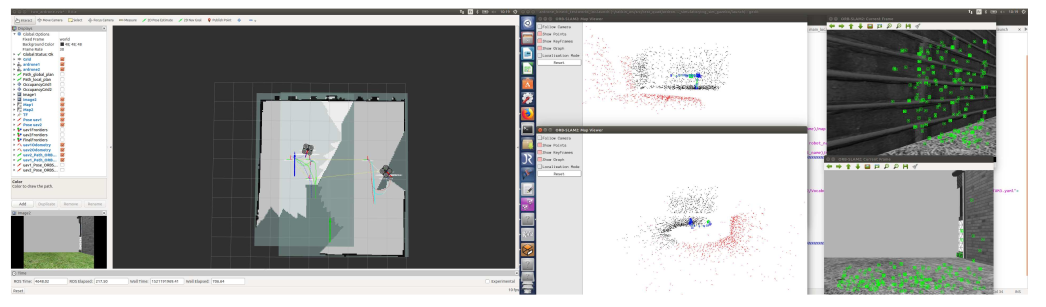
\includegraphics[scale=0.3]{assets/3_23.png}
    \caption{Two UAVs navigation using ORB-SLAM2. Rviz image (left) shows, for each UAV, the constructed 2D occupancy grid map, its estimated trajectory and the corresponding ground truth. The point cloud (middle) represent the sparse reconstruction of the environment made by each UAV. And, the green markers (right) represent the features computed by each UAV to perform localization.}
    \label{fig:3.23}
\end{figure}
Each robot performs SLAM where it constructs its map in its local reference frame $^WF_i$ , and estimates its relative pose $\mathbf{p}_i$ within it. Then, the fleet performs cooperative explo- ration using some specific information exchanged among UAVs. But, these information have to be in a common reference frame. Therefore, information such as the pose $\mathbf{p}_i$ and the frontier points $\mathbf{f}_{i,j}$ are necessarily transformed into the global reference frame $^0W$ before being exchanged. Hence, the \textit{leader} makes all the needed computation and sends back to the \textit{explorers} the targets in $^0W$. When a robot receives its assigned goal, it transforms it into $^WF_i$ to plan a path to it.\\\\
To perform a transformation from local reference $^WF_i$ to global one $^0W$, the robot has to know – at least – its initial pose w.r.t. $^0W$. As explained in Section 5.2 of Chapter 1, the global reference frame of the environment is initialized such that it coincides with the local reference frame of the first group-\textit{leader} in the fleet which is UAV$_1$ in the considered example of Equation \ref{eq:3.9}.
\begin{equation}\label{eq:3.9}
    ^0W\equiv ^WF_1,
\end{equation}
Then, by detecting this robot using tags mounted on it, the other robots are able to estimate their respective transform to it $^{F_j}\begin{bmatrix}\mathbf{R} & \mathbf{t}\end{bmatrix}_{F_1}, j \in [2..n_c]$. For simulation evaluations, the information of transform – computed while detecting the tag – are assumed to be known. Figure \ref{fig:3.24} shows the exploration rate evolution during the exploration mission while using ORB-SLAM2 as the relative localization approach. The mission time using ORB-SLAM2 is reduced by $43\%$ for 2 UAVs instead of 1 UAV.
\begin{figure}[H]
    \centering
    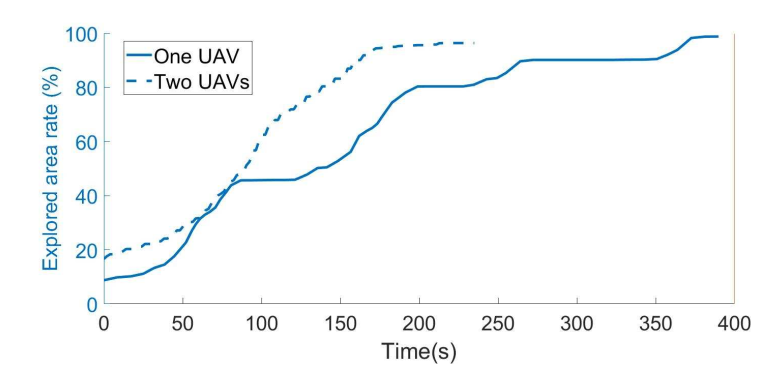
\includegraphics[scale=0.4]{assets/3_24.png}
    \caption{Explored area rate evolution during exploration mission with one and two UAVs while performing ORB-SLAM2 by each UAV.}
    \label{fig:3.24}
\end{figure}
The exploration time when using a relative localization (See Figure \ref{fig:3.24}) is relatively important compared to the exploration without SLAM (See Figure \ref{fig:3.18}) since the velocity has been considerably reduced.
\section{Conclusion}
In this chapter, we presented a state of the art of multi-robot exploration mission including the strategy used to assign a robot to a target and an utility function adopted to estimate the interest of reaching it. Then, we introduced an exploration strategy based on the group-\textit{leader} decision making. The robot-to-target assignment is performed using a novel utility function. This function makes a trade-off between fast exploration and getting a detailed grid map, and also takes into account the distance of each robot in the group from the unexplored set of targets. Also, we propose to schedule the information gain in order to efficiently spread the UAVs into the environment. Moreover, the strategy adopted exchanges the frontier points instead of a whole copy of the local map.\\\\
Results show that the proposed cooperative exploration strategy minimizes the global exploration time by $25\%$ for 2 UAVs and by $30\%$ for 3 UAVs, while minimizing the average traveled distance by each UAV by $55\%$ for 2 UAVs and by $62\%$ for 3 UAVs. Furthermore, the strategy was evaluated using a relative localization algorithm where the exploration time was reduced by $43\%$ for 2 UAVs instead of 1 UAV.
%------------------CHAPTER 4------------------------------------------------%
\chapter{Inter-robot communication}
\section{Introduction}
A critical subject in multi-robot systems is the communication among robots. This feature is used for coordination and to share specific information. A fleet can be deployed in several missions within relatively difficult and hostile areas. But, these environments may have no pre-existing network infrastructure, in addition to non ideal communication links.\\\\
This chapter highlights one of the most challenging points in MRS, which is the inter- robot communication. This problem can be addressed from different perspectives; but, we have chosen to study two sub-problems, which are: network typology, and network topology and strategy for MRS robustness.
\section{Network classification}
The network is used to link between different entities and to establish possible communi- cation between them. Several network types exist and can be classified in different ways.
\subsection{Infrastructure versus infrastructureless mode}
To manage network infrastructure, the existed modes can be classified into two major categories [Äřlker Bekmezci et al., 2013, Hayat et al., 2015]. The first kind is the infrastructure mode, which can be called Access Point (AP) mode, and the second kind is
the infrastructureless mode named Ad Hoc mode (See Figure \ref{fig:4.1}). In the AP mode, the UAV-to-UAV communication is realized through the infrastructure (AP, routers, etc.), unlike the Ad Hoc mode in which nodes communicate directly with each other. The Ad Hoc mode is also called peer to peer mode. The Ad Hoc network can grow into another peer to peer mode called mesh network by enabling multi-hop capability. Indeed, the Ad- Hoc networks do not have any inherent capability for multi-hop. Nodes communicate with each other when they are within one another’s communication range. Whereas, in mesh networks, nodes are able to communicate directly or through one or more intermediate nodes.
\begin{figure}[H]
    \centering
    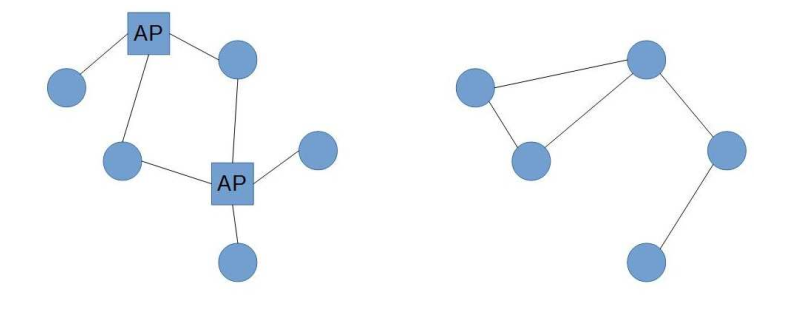
\includegraphics[scale=0.4]{assets/4_1.png}
    \caption{Infrastructure (left) and infrastructureless (right) mode.}
    \label{fig:4.1}
\end{figure}
\begin{table}[H]
    \centering
    \caption{Infrastructure versus Infrastructureless mode.}
    \label{tab:4.1}
    \begin{tabular}{|l|p{4.5cm}|p{4.5cm}|}\hline
                               & \textbf{Infrastructure mode}      & \textbf{Infrastructureless mode}
        \\\hline
        \textbf{Advantages}    & Reliability of communication      & Direct connection to each other,
        easy to set up, robust to node fail-
        ure, allow expansion and modifica-
        tion in network topology.                                                                     \\\hline
        \textbf{Disadvantages} & Expensive, complicated hardware,
        range restriction.     & Redundancy in network connection,
        difficult maintenance.                                                                          \\\hline
        \textbf{Standard}      & 802.11                            & 802.11, 802.15, 802.16           \\\hline
    \end{tabular}
\end{table}
Originally, robots have to perform their tasks in environments without network infras- tructure. In fact, they exchange information when they act as routers and as APs. So, the MRS system can be seen as a mobile Ad Hoc network in a communication point of view.
\subsection{Ad Hoc network classification}
Ad Hoc Network is the commonly used network to manage multi-robot communication. With this network, each robot can move freely and forward packets to and from each other depending on the mode of distribution of data [Bouachir, 2014]. This network is characterized by sophisticated quality of service in which routing protocol determines the optimal path of the information taking into account the frequent change of the topology. Added to that, it is cheaper to realize this kind of network instead of others (satellite, cellular, etc.).\\\\
The Ad Hoc network can be classified into three main categories which are Mobile Ah doc NETwork (MANET), Vehicular Ah doc NETwork (VANET), and Flying Ad hoc NETworks (FANET). For multi-UAV system, generally, the FANET model is adopted. Table \ref{tab:4.2} details each category’s characteristics [Äřlker Bekmezci et al., 2013, Maistrenko et al., 2016] and also analyses our model’s expectations.
\begin{table}[H]
    \centering
    \caption{Comparison between MANET, VANET, FANET and our model’s network expectation.}
    \label{tab:4.2}
    \begin{tabular}{|p{2.8cm}|p{1.5cm}|p{1.5cm}|p{1.8cm}|p{1.8cm}|}\hline
        \textbf{Characteristics}                                     & \textbf{MANET}                                    & \textbf{VANET}                 & \textbf{FANET}                                                       & \textbf{Our model expectation}
        \\\hline
        \textbf{Mobility}                                            & Men in certain terrain                            & Vehicle in highway             & Plane in 3D plan                                                     & 3D                             \\\hline
        \textbf{Mobility degree}                                     & $+$                                               & $+$                            & $++$                                                                 & $++$                           \\\hline
        \textbf{Mobility model}                                      & Random way points with random direction and speed & Highly predictable in roads    & Not predetermined (random UAV movement model, pheromone based model) & Predictable                    \\\hline
        \textbf{Topology changes}                                    & $+$                                               & $+$                            & $++$                                                                 & $++$                           \\\hline
        \textbf{Distance between nodes}                              & $+$                                               & $+$                            & $++$                                                                 & $+$                            \\\hline
        \textbf{Node density}                                        & $++$                                              & $++$                           & $+$                                                                  & $+$                            \\\hline
        \textbf{Radio propagation model}                             & Rare presence of line of sight                    & Rare presence of line of sight & Frequent presence of line of sight                                   & Always presence of line sight  \\\hline
        \textbf{Power consumption and life time computational power} & $+$                                               & $+$                            & $++$                                                                 & $++$                           \\\hline
        \textbf{Standard}                                            & IEEE 802.11, 802.15, 802.15.4, 802.16 and 802.20  & IEEE 802.11p                   & IEEE 802.11                                                          & ?                              \\\hline
    \end{tabular}
\end{table}
The comparison shows that FANET is the closest network to our model’s expectations. Hence, among the available standards for this kind of network, IEEE 802.11b and IEEE 802.11g provide high data rates and are typically used for multi-robot systems.
\subsection{Network topology classification}
The network topology defines the starting points, the endpoints and the paths of the information in the network. Given target points, the topology defines all possible paths to reach them.\\\\
From a software point of view, the network an be mainly classified in three topology (See Figure \ref{fig:4.2}\footnote{Source: From user 1983 on Wikipedia. Licensed CC BY-SA}):
\begin{figure}[H]
    \centering
    \includegraphics[scale=0.4]{assets/4_2.png}
    \caption{Centralized (left), decentralized (middle) and distributed (right) networks.}
    \label{fig:4.2}
\end{figure}
\begin{itemize}
    \item Centralized network: It is the most used topology [Morgenthaler et al., 2012], [Froster et al., 2013b]. All nodes - also called stations - are connected to each other via a centralized hub. That is when a node needs to send an information to another one, the data necessarily pass through the central node to be routed to its destination. If the central node is out of service or unreachable, no data can be transmitted which makes this topology vulnerable to node failure.
    \item Decentralized network: This topology is considered as a set of centralized networks connected together [Fox et al., 2003], [Brand et al., 2014]. One central hub is employed for every little group of nodes to send and receive the information. If a hub fails, nodes which are direactly relied to it become inaccessible.
    \item Distributed network: This topology contains nodes that are connected to each others. Unlike the centralized topology, several paths are possible to reach one destination. Also, nodes are not affected by one node's failure. This allows to increase the survivability and to decrease the vulnerability of the network. The distributed topology is attractive to ensure reliable network [Cunningham et al., 2010]. Nevertheless, it is quite difficult to reach and to realize in reality, and the simulation are not fully distributed [Waharte et al., 2009], [Cameron and Trigoni, 2009], [Scherer et al., 2015]. This is because all processing and decision making have to be on-board the robot whichs requires an important memory and a heavy computation.
\end{itemize}
\section{Network typology}
The typology of the network represents its type and, accordingly, the characteristics introduced.
\subsection{Related work}
MRS communication is a critical problem to tackle in the robotics community. In the last decade, the great progress in wireless technologies and MRS has created a growing interest for inter-robot communication. Hence, different methods have been proposed.\\\\
To face disaster scenarios such as fire in an industrial warehouse, authors in [Witkowski et al., 2008] propose to use Wireless LAN, Bluetooth and ZigBee to form an Ad- Hoc network. Some robots of the fleet form the network infrastructure to support communication.\\\\
Authors in [Morgenthaler et al., 2012] use two network standards to build a multi-UAV system. A IEEE 802.11s wireless mesh network is build using UAVs carrying mesh nodes directly connected to the flight electronics. Each of these mesh nodes acts as an AP in order to form an IEEE 802.11g.\\\\
A methodology that profiles the wireless links for Linux-based networked aerial vehicles is presented in [Kuschnig et al., 2012]. The approach includes two options to collect link quality information and to monitor the 802.11 wireless interface.\\\\
An evaluation of the standard 802.11a used between an UAV and an AP is performed in [Kuschnig et al., 2012]. Results show that the Received Signal Strength (RSS) for the downlink decreases with the distance to the AP but remains at an acceptable level as well as the throughput.\\\\
Knowing that the visible light spectrum is much wider than the Radio Frequency spectrum, it seems interesting to uptake Visible Light Communication (VLC) based on Light Emitting Diodes (LEDs). IEEE has developed the 802.15.7 standard for short range communication using visible light. Authors in [Wang et al., 2014] introduce a bidirectional communication using Open VLC. This solution hardware needs a Beagle Bone Black (BBB) board and a font transceiver that employs a single LED to both transmit and receive. The solution is implemented on Linux driver that communicates directly with the LED front-end and the Linux networking stack. The main idea to reuse the same LED for both Transmitting (TX mode) and Receiving Light signal (RX mode) is that when a node is transmitting data, the other node can expect the LOW symbol of the bit 0 and makes use of this time to switch his mode from RX to TX and transmit data.\\\\
The Zigbee – based on IEEE 802.15.4 – is a protocol of high level which is particularly useful for short communication range and low consumption. Several UAVs’ application use this network [Asadpour et al., 2014]. Communication can be made under three frequency bands depending on the chipset type: 868MHz for a bit rate of 20 kbps, 915MHz for 40 kbps and 2.4GHz for 250 kbps.\\\\
Authors in [Vidal et al., 2015] adopt different sized groups composed of tactical UAVs and UAVs moving in delimited geographical areas. Virtualization techniques are used to adapt the upgrade of any function, which allows the flexibility in heterogeneous services.\\\\
In a search and rescue mission, for example, authors in [Scherer et al., 2015] propose to do real-time streaming between UAVs over a large distance. The mission is divided into five principle phases: The pre-planning to define the best paths in the search area allowing to reduce the time of the mission then searching by just following the predefined way- points; the detection of the target and sending the new plans to the others, followed by the repositioning by setting a multi hop link to evaluate the situation by the base station and finally, the streaming of the video.\\\\
The multi-UAV, moving in a three dimensional space, need sophisticated transmission systems to ensure flexibility. In [Scherer et al., 2015], an omni-directional isotropic antenna is fixed on the base station and on all the deployed heterogeneous UAVs. For data exchange, the standard IEEE 802.11s mesh technology is used.\\\\
Authors in [Hayat et al., 2015] present a performances comparison between the stan- dard IEEE 802.11n and the IEEE 802.11ac in a multi hop network. Both networks were experimented in indoor and outdoor environment, and in two mode, the access point mode (AP)/infrastructure mode and the mesh mode regarding throughput and fairness. In indoor experiments, for an infrastructure mode, the 802.11ac shows improved performances in both TCP and UDP throughput, and packet loss for UDP traffic. In outdoor experiments, for infrastructure mode, the throughput of 802.11n is three time higher than that of 802.11a however, the link quality drops more steeply. For mesh mode, 802.11n achieves higher throughput at close range but drops faster as soon as date rate gets higher and the range longer. The recorded throughput for mesh network is lower than infrastructure mode due to the longer inter-packet transmission times.\\\\
To face issues of maintenance connectivity, collision avoidance, robustness to failure and area coverage improvement, authors in [Ghedini et al., 2018] propose a novel model that provides more efficient network topologies.\\\\
In [Harms et al., 2018], a new communication layer is proposed to deal with networks that requires a high bandwidth. For that, some mechanism are used to buffer messages, to compress data or to react to unexpected situations.\\\\
Table \ref{tab:4.3} lists some standards used in multi-robot systems. For each standard, we detail the concerned layer in the OSI model, its characteristics, the resulting performances, and the hardware and software used for experiments.
\end{document}